% \documentclass[journal=jacsat, manuscript=article]{achemso}
\documentclass[pdftex,11pt,a4paper,twocolumn]{scrartcl}
\usepackage{enumerate} 
\usepackage{listings}
\usepackage{algorithm} 
\usepackage{algorithmic}
\usepackage{amsmath}
\usepackage{mathtools}
\usepackage{setspace}
\usepackage[pdftex]{graphicx}
\usepackage{graphics}
\usepackage{indentfirst} 
\setlength{\parindent}{15pt}
\setlength{\parskip}{5pt}
\usepackage{multicol}
\setlength{\columnsep}{1cm}
\usepackage{fullpage}
\usepackage{hyperref}


\author{Philip Steele}
\author{Vangelis Dimopoulos \\ Philip Steele}
\title{Comparative Analysis between Graph Generating and Sub-Sampling Algorithms using Twitter Data\footnote{All files for this project, including this document, can be found at \url{https://github.com/pdsteele/socialNetworksProject}}}
\date{}

\begin{document}
\onecolumn
\maketitle
\bibliographystyle{ieeetr}  
\singlespacing

\section*{Abstract}

Social network analyses have sparked a large source of interest over the last decade. The high computational complexity of analyzing these rather large social network graphs, along with the API restrictions imposed on data collection, have served as large barriers to entry for analysis. To address these issues, researchers have explored many techniques for taking sub-samples of large input graphs. Our research seeks to evaluate which of these techniques are the most effective at generating graphs that are representative of the population of the input graph.

After finding an appropriate sub-sampling method, we concentrate our efforts in exploring and modifying several graph generation algorithms to simulate real-world directed graphs. Using the induced sub-samples as our basis for generation, we compare the new graphs using several measures that characterize the structure of directed graphs. Our results indicate that while they closely match several characteristics from the original graph (including the in-, out-, and reciprocal-degree distributions, diameter, and hop plot), the clustering coefficients and proportion of edges that are reciprocal were generated with mixed results. Several recommendations are then made for future work to improve upon these results. 

\newpage

\tableofcontents

\newpage

\twocolumn
\section{Introduction}
%\addcontentsline{toc}{section}{Introduction}

Analyzing real-world networks can be a challenge. Their gigantic sizes, application programming interface (API) call limitations, and high computational complexity are all restrictions that bar individuals from conducting analyses on these networks. To bypass this issue, however, researchers designed algorithms to generate graphs whose structure emulates that of their real-world counterparts. Most of the algorithms, including the Erdos-Renyi, Preferential Attachment, and Chung-Lu models, have been designed with undirected networks (like LinkedIn or Facebook). Our goal was to substantially modify these algorithms for directed networks, like Twitter, and to analyze their overall accuracy.


First we sub-sample an existing directed-graph (Twitter data set) to find smaller and more manageable representative graphs using two main methodologies: Random Selection and Random Walk (RW) discussed in \cite{sampling}. Their findings indicate that for the ``scale-down" goal, whose objective reduces the overall size of the graph while maintaining its structural properties, the random walk (RW) methodology is most accurate for undirected graphs. Using a Twitter data set from \cite{snap} in conjunction with the RW methodology, we elaborate on the various graph generating methods and discuss our directed-graph modifications. After elaborating on each methods strength's and weaknesses, we compare statistics from generated directed graphs. Finally we make our recommendation as to which generation method, if any, can accurately simulate a directed graph (in our case, Twitter).

%Added this for additional clarification purposes.
For those unfamiliar with the anatomy of Twitter, we first cover the basics of the micro-blogging webpage. The relationship between users is a directed graph defined by either ``Following" or ``Followers". If User A connects to User B, or a directed edge from A to B, we say that User A is following User B (or receives all of the tweets made by User B) and User B has the Follower User A. Note this is a directed graph where User B does not have to reciprocate the ``Following" action with User A; therefore, User B can select to avoid receiving User A's tweets. Each user has the option of posting a limited character ``tweet", in which their followers can read and keep up with the users blog. If a tweet contains a level of information worth repeating, a different twitter user could re-tweet the content to all of their followers. While the scope of our analysis does not include tweeting and re-tweeting characteristics of this network, our findings of simulating directed networks can apply directly to the numerous applicable settings.

\section{Random Subgraph Selection Methodology}
%\addcontentsline{toc}{section}{Random Subgraph Selection Methodology}
Algorithms used to graph measurements can be immensely computationally intensive for real world graphs \cite{sampling}. Therefore, using a sub sample of this real graph, directed or undirected, will allow for a more efficient computation; a crucial factor in our analyses. Leskovec and Faloutsos defined two main goals for sampling. The first of which is the Back-in-Time goal, which aims to obtain a sample that appears similar to the graph when it was the size of the sample. The other is the Scale-Down goal, which aims to get a sample from the graph with all the representative characteristics of the original. For our purposes, the latter goal is most desirable. Of the algorithms tested in \cite{sampling} for undirected graphs, with the Scale-Down goal in mind, the strongest algorithm satisfying this was a method called Random-Walk. In the following section, we provide a definition for the Random-Walk, we modify this goal for directed graphs, and provide an alternate Random-Edge selection for comparison.

\subsection{Random Selection}
%\addcontentsline{toc}{subsection}{Random Selection}
%Van
In the random selection method, we iterate through every edge in the full graph and accept the edge with probability $p$ or go back to the start with probability $(1-p)$. This can be implemented through a $Bernoulli(p)$ trial. In short, we generate a random variable, $u \sim U(0,1)$ and if this $u \le p$, then we select the listed edge, otherwise we reject the edge and continue. For our purposes, we selected random samples at rates of $p_1 = 25\%$, $p_2 = 50\%$, for reasons that coincide with the percentage requirements described in the following section.


\subsection{Random Walk Sampling}
%\addcontentsline{toc}{subsection}{Random Walk Sampling}
%Van
The random walk (RW) sampling, as suggested in \cite{sampling}, first selects a start node, then uses the similar $Bernoulli(p)$ trial, where $p$ represents the probability of returning to the start node. It follows that with probability $(1-p)$, the algorithm selects an available directed edge to another node then ``walks" to the next node, where the $Bernoulli(p)$ trial is performed again. This is performed either until a specific percentage of the original number of edges is recorded, or until $100*n$ iterations are performed (where $n$ is the number of edges), at which point the algorithm terminates. Leskovec and Faloutsos claim $p=0.15$ is a suitable probability for returning to the starting node, so we incorporated this reported percentage into our model. Since we are working with directed graphs, it is especially important to select a node that has many ``out" connections, which allows for many different random walks across the graph. Finally, the authors of \cite{sampling} indicate that a representative sample can not be obtained with fewer than $25\%$ of the nodes. Therefore, as a basis for comparison, we set our desired percentages to both $25\%$ and $50\%$ of the original data sets as terminating conditions. The other terminating condition remains unchanged.

\section{Directed Graph Generation}
%\addcontentsline{toc}{section}{Directed Graph Generation}
%Van and Phil
The next major consideration of this paper is the accuracy of directed graph generators. In this section, we briefly review several methods that can be used for generating graphs based on an input graph's characteristics. Then, after reviewing our reasons for selecting particular algorithms, we present modifications for the Transitive-Chung-Lu algorithm to produce directed graphs, and the Fast-Reciprocal-Directed-Graph generation algorithm.

\subsection{Background}

While there are many techniques for generating undirected graphs, such as the Erdos-Renyi model, the Kronecker Product Graph model (KPGM), or the Chung-Lu model, there is less emphasis placed on their direct graph counterparts. Moreover, many generators are not designed to replicate real-world graphs, but to simply generate a graph that matches a desired degree distribution. In order to use an algorithm that generates directed graphs that match all desired characteristics, it is first necessary to establish a strong underlying model that we can modify accordingly.

First, it is clear that Erdos-Renyi is an insufficient model for this purpose. Since it does not use an input graph for generation and it does not generate a power-law degree distribution, it does not replicate the degree distribution of any real world graphs. To address this, exponential random graph models were developed to allow the generated graphs to have a matching degree/clustering distribution. This modified process, however, is extremely resource intensive and cannot be used to generate networks with more than a few thousand nodes.

%Van: KPGM - http://cs.stanford.edu/people/jure/pubs/kronecker-jmlr10.pdf
%Parameters - Maximum Likelihood

The Chung-Lu model, an extension of the Erdos-Renyi model, utilizes the exact degree distribution of a real-world graph for generating undirected graphs. The algorithm first uses an empirical cumulative distribution function for the degree distribution, generates a $U_i \sim U(0,1)$ random variable, and uses the inverse cumulative distribution function $D_i = F^{-1}(U_i)$ to select a node. With large sampling, the Chung-Lu generates a graph whose expected degree distribution matches that of the original. 

In contrast, the Kronecker Product Graph Model uses a $2\times 2$ initiator matrix of parameters where the elements on the principle diagonal represent transitions within a community and the elements on the off-diagonal the transition between communities. The matrix is found using a maximum-likelihood function, as described in \cite{fgls}. After an initiator matrix, say $A_{m\times n}$ is generated, the Kronecker product of the matrix is taken by itself. That is:

\tiny
\begin{equation*}
A^{\prime}_{m^2\times n^2} = A_{m\times n} \otimes A_{m\times n} =
\end{equation*}
\begin{equation*}
    \begin{bmatrix}
       a_{1,1}*A_{m\times n} & \dots & a_{1,n}*A_{m\times n} \\[0.3em]
       \vdots & \ddots  & \vdots \\[0.3em]
        a_{m,1}*A_{m\times n} & \dots & a_{m,n}*A_{m\times n}
     \end{bmatrix}
\end{equation*}

\normalsize

This operation is performed using the resulting matrix and the original $log(N)$ times, where $N$ corresponds to the number of nodes in the matrix. The resulting matrix $P$ with dimensions $2^{log(N)}\times 2^{log(N)}$ generates the likelihood or probability of drawing an edge between two nodes \cite{fgls}.
 
Both of these models are much faster than exponential random graph models, and they accurately model the degree distributions of an undirected input graph. Moreover, they are capable of replicating the diameter of small-diameter graphs. However, they do not accurately capture the clustering of a real-world graph, and Kronecker Product Graph Model is computationally intensive, requiring quite a bit of computer memory.

To address these issues, the authors of \cite{fgls} modified the Chung-Lu algorithm to create the Transitive Chung-Lu algorithm. This modified process addressed an edge collision problem from the original to improve the accuracy, and introduced a `random triangle' parameter to the model. This enables the clustering of the undirected input graph to be accurately emulated. Furthermore, this parameter allows an additional probability of creating new transitive edges across a pair of nodes connected by a two-hop path (similar to a re-tweet in Twitter). In contrast, the original Chung-Lu model employs a simple `random surfer' method to dictate edge generation, similar to the PageRank algorithm. 

In \cite{fgls}, the authors found that the Transitive Chung-Lu algorithm was capable of replicating the degree distribution, the clustering coefficients, and the hop plot of an undirected input graph. Moreover, it was able to generate these graphs significantly faster than any of the prior researched methods. It can also be performed as an additional refining mechanism after a previous algorithm is used, with the goal of improving the clustering coefficient distribution. For the reasons listed above, we have chosen to modify the Transitive Chung-Lu algorithm to generate directed graphs based our existing Twitter data set's characteristics as the corresponding input.

In the following sections, we cover the changes to Chung-Lu and Transitive Chung-Lu needed to generate directed edges. We also cover another algorithm based on CL, the Fast Reciprocal Directed Generator, and discuss how it was modified in \cite{FRDG} for directed graphs. We then briefly discuss the differences between these approaches, and the potential to use them sequentially for the most accurate graph generation. 

\subsection{Modified Chung-Lu}
%\addcontentsline{toc}{subsection}{Modified Transitive Chung-Lu}
%Van - Algorithm and approach
%Phil - Otherwise

In order to modify the Transitive Chung-Lu algorithm, it is first necessary to modify the base Chung-Lu Algorithm. The basis for the algorithm in the undirected case lies in an underlying degree distribution of the data set. This is then converted to an empirical cumulative distribution function, allowing us to select a probability $p \sim U(0,1)$ where $U(0,1)$ is a uniform random variable ranging from $0$ to $1$. Converting this function to accept input and correctly modify a directed graph requires obtaining both the in and out degree distributions from the underlying directed graphs. 

In order to generate the tuples $(v_i,v_j)$ (which represents a directed node-to-node connection $v_i \rightarrow v_j$) for the directed case, the in and out degree distributions are required to properly select an in-degree for each $v_j$ and out-degree for each $v_i$. More specifically, the degree distributions are used to generate ECDFs, which are sampled from up to $m$ times (where $m$ is the number of edges in the graph). By taking $m$ random samples, a node with in-degree $i$ is selected about $i$ times as a target node, and a node with out-degree $j$ is selected about $j$ times as a source node. 

The last major change required was for the queue that Chung-Lu uses. If Chung-Lu generates an edge that is already in the graph, then it queues up the nodes of that edge, and re-pairs them for another edge in the next two iterations. However, with the notion of directed edges, this no longer works. To address this, our implementation queues a tuple of the node number and its type (target or source). Then when a node is de-queued, it is re-paired with a node that is randomly selected from the correct ECDF (i.e., if a target node is de-queued, a new source node is drawn randomly using the out-degree ECDF). 

The detailed modification to the algorithm is shown below in Algorithm~\ref{fig:CL}. With the Chung-Lu properly modified, the Transitive Chung-Lu can now be modified with similar changes to emulate the clustering distribution of directed graphs. 

\begin{algorithm}[width=\columnwidth, b]
\begin{minipage}{\columnwidth}
\begin{algorithmic} 
%\REQUIRE $n \geq 0 \vee x \neq 0$
%\ENSURE $y = x^n$
\STATE $\mbox{Edges = \{\} }$
\STATE $\mbox{Queue = Queue() }$
\FOR{$i=1:TotalEdges$} 
\IF{$\mbox{Queue.isEmpty()}$}
\STATE $v_j = \mbox{NodeSelect(InDegreeECDF)}$
\STATE $v_i = \mbox{NodeSelect(OutDegreeECDF)}$
\ELSE
\STATE $temp = \mbox{Queue.dequeue()}$
\STATE $node = temp[0]$
\STATE $type = temp[1]$
\IF{$type==0$}
\STATE $v_i = node$
\STATE $v_j = \mbox{NodeSelect(InDegreeECDF)}$ 
\ELSE
\STATE $v_j = node$
\STATE $v_i = \mbox{NodeSelect(OutDegreeECDF)}$ 
\ENDIF
\ENDIF
%\WHILE{$N \neq 0$}

\IF{$(v_i,v_j) \not\in$ Edges}
\STATE $\mbox{Edges.add(}v_i,v_j\mbox{)}$
\ELSE
\STATE $\mbox{Queue.enqueue}(v_i,0)$
\STATE $\mbox{Queue.enqueue}(v_j,1)$
\ENDIF
\ENDFOR
\RETURN Edges
%\ENDWHILE
\end{algorithmic}
\caption{Directed Chung-Lu}
\label{fig:CL}
\end{minipage}
\end{algorithm}


\subsection{Modified Transitive Chung-Lu}

Before addressing how the algorithm is modified it is necessary to discuss a key difference between Transitive Chung-Lu and CL. First, Transitive Chung-Lu is not a graph generator by itself. It re-lays the edges of a generated graph in the order that they were initially generated, and it uses the degree and clustering distributions of the undirected input graph to influence how it re-lays the edges. Therefore, running it requires generating a graph using Chung-Lu or another algorithm beforehand. While this does not require modification for directed graphs, it is an important detail for implementation (especially when dealing with the order that edges were generated by another algorithm). 

Another key difference between Chung-Lu and Transitive Chung-Lu is that the latter utilizes priority queues when it generates a duplicate edge in the graph. This reduces the likelihood of cycling the same edge, and ensures accurate modeling of high degree nodes \cite{fgls}. Similar to the Chung-Lu algorithm, this requires adjustment for the directed graph case. Our adjustment is handled similarly by queuing tuples that contain a node number and a boolean to indicate whether they are a source or target node (e.g., 0 for source and 1 for target). Then when the nodes are de-queued, they are re-paired with another randomly selected node of the opposite type. If there are no elements in the queue, then a $Bernoulli(.5)$ is generated to determine whether to randomly select a source or a target. However, there are now two methods for randomly selecting nodes. 

The biggest difference between Transitive Chung-Lu and Chung-Lu is the random triangle parameter $p$. In the undirected case, for every edge generated, there is a $p$ chance that the source node will be selected to be a node that is two hops away from the (already) selected target node. Otherwise, the source node will be selected using the ECDF. In other words, after selecting a target node $v_j$, then with probability $p$, the algorithm selects a node $v_k$ randomly from all edges $(k,j) \in E$. Then it selects the source node, $v_i$, randomly from all edges $(i,k) \in E$. 

For the directed case, this must be able to start from a source node or a target node, and randomly select a node of the opposite type that is two hops away. For example, source node $v_i$ may be used for randomly selecting $(v_i, v_k)$ then $(v_k, v_j)$, or target node $v_j$ may be used for randomly selecting $(v_k,v_j)$ then $(v_i,v_k)$. 

The full directed version of this algorithm appears in Algorithm~\ref{fig:TCL}. The following section shows how the algorithm must also be modified to select the probability of creating a two-hop edge.  


\begin{algorithm}[H]
\begin{minipage}{\columnwidth}
\begin{algorithmic} 
%\REQUIRE $n \geq 0 \vee x \neq 0$
%\ENSURE $y = x^n$
\STATE $\mbox{Edges = Chung-Lu }$
\STATE $\mbox{PQueue = PriorityQueue() }$
\STATE $p = \mbox{learnP()}$
\FOR{$i=1:TotalEdges$} 
\IF{$\mbox{PQueue.isEmpty()}$}
\STATE $\mbox{d = Bernoulli(p)}$
\IF{$d=0$}
\STATE $nodeType = 0$
\STATE $v_i = \mbox{NodeSelect(OutDegreeCDF)}$
\ELSE
\STATE $nodeType = 1$
\STATE $v_j = \mbox{NodeSelect(InDegreeCDF)}$
\ENDIF
\ELSE %for pq.empty if statement 
\STATE $temp = \mbox{PQueue.dequeue()}$
\STATE $node = temp.data[0]$
\STATE $nodeType = temp.data[1]$
\ENDIF

\STATE $\mbox{r = Bernoulli(p)}$
\IF{$\mbox{nodeType}=1$}
\IF{$r=1$}
\STATE $v_k = \mbox{UniformSelect(Edges,}v_j)$
\STATE $v_i = \mbox{UniformSelect(Edges,}v_k)$
\ELSE
\STATE $v_i = \mbox{NodeSelect(OutDegreeCDF)}$
\ENDIF
\ELSE
\IF{$r=1$}
\STATE $v_k = \mbox{UniformSelect(RevEdges,}v_i)$
\STATE $v_j = \mbox{UniformSelect(RevEdges,}v_k)$
\ELSE
\STATE $v_j = \mbox{NodeSelect(InDegreeCDF)}$
\ENDIF
\ENDIF
%\WHILE{$N \neq 0$}
\IF{$(v_i,v_j) \not\in$ Edges}
\STATE $\mbox{Edges.add(}v_i,v_j\mbox{)}$
\STATE $\mbox{Edges.delete(EarliestAddedNode())}$
\ELSE
\STATE $\mbox{PQueue.enqueue}((v_i,0),outDegreePDF_i)$
\STATE $\mbox{PQueue.enqueue}((v_j,1),inDegreePDF_j)$
\ENDIF
\ENDFOR
\RETURN Edges
\end{algorithmic}
\caption{Directed Transitive Chung-Lu}
\label{fig:TCL}
\end{minipage}
\end{algorithm}



\subsubsection{Selecting Random Triangle Parameter $p$}

In the undirected version of this algorithm, the probability of creating a two-hop edge, $p$, is selected using an expectation maximization algorithm. The original form is shown in \cite{fgls}. In short, it initializes $p$ as an arbitrary number between 0 and 1 (.5 works well to minimize iterations to convergence), and then performs the following calculation to update $p$:

\tiny
\begin{equation*}
p^{t+1} = \frac{1}{|S|} \sum_{e_{i,j} \in S} \frac{p^t(\sum_{v_k \in e_{j,*}} \frac{I(v_i \in e_{k,*})}{D_{j,j}*D_{k,k}})}{p^t(\sum_{v_k \in e_{j,*}} \frac{I(v_i \in e_{k,*})}{D_{j,j}*D_{k,k}}) + (1-p^t)(\pi(i))}
\end{equation*}
\normalsize

Where $S$ is a large sample of edges (10000 is sufficient), $D_{i,i}$ is the degree of the $i^{th}$ node, $I$ is an indicator function, and $\pi(i) = \frac{D_{i,i}}{2M}$. Each edge is sampled by selecting a node from the ECDF of the degree distribution, and then randomly selecting an incident edge.

In order to modify this algorithm for the directed input graph case, the first node, $v_i$,  selected for each iteration must be drawn from the ECDF of a degree distribution (selected by coin flip, similar to de-queuing an element in TCL). Then a one-hop node, $v_j$, must be selected from one of the edges that the first node is incident to. Finally, all other edges from the second node are iterated through for the list of available two-hop nodes. If any nodes, $v_k$, are connected to the first node, then it increases a sum (initialized at 0) by 

\tiny
$$\frac{1}{inDeg_{j} + outDeg_{j}}*\frac{1}{inDeg_{k} + outDeg_{k}}$$ 
\normalsize

The equation from the undirected case now becomes:

\small
\begin{equation*}
p^{t+1} = \frac{1}{|S|} \sum_{e_{i,j} \in S} \frac{\alpha}{\alpha + \beta }
\end{equation*}
\normalsize

\newpage 

Where: 
\tiny
\begin{align*}
&\alpha = p^t(\sum_{v_k \in e_{j,*}} \frac{I(v_i \in e_{k,*})}{(inDeg_{j} + outDeg_{j})*(inDeg_{k} + outDeg_{k})}) \\
\small
&\beta = (1-p^t)(\pi_{in}(i) + \pi_out(i)) \\
&\pi_{in}(i) = \frac{inDeg_{i}}{M} \\
&\pi_{out}(i) = \frac{outDeg_{i}}{M} \\
\end{align*}

\normalsize

The full algorithm for selecting $p$ is shown in Appendix~\ref{sec:pLearn}. Our TCL implementation (including the expectation maximization algorithm and directed Chung-Lu graph generation) is shown in Appendix Section~\ref{sec:TCL}. 

\subsection{Fast Reciprocal Directed Graph}
%\addcontentsline{toc}{subsection}{Fast Reciprocal Directed Graph}
%phil 
The Fast Reciprocal Directed Graph generation algorithm was developed by a team of Sandia researchers in 2013 as a scalable null model for directed graph generation \cite{FRDG}. Similar to the authors of this paper, they aimed to use the Chung-Lu methodology with directed graphs; but, they also sought to dramatically reduce the run-time while modeling the generation of low degree nodes more accurately. Moreover, the team also noticed that no models currently were modeling the reciprocal degree distribution (the distribution of nodes that have edges to each other), and aimed to model this distribution as well. To evaluate the proportion of edges are reciprocal, \cite{FRDG} use a reciprocity measure, defined as:

\small
$$r = \frac{\sum_{d=1}^{d_{max}} d*n_d}{m} = \frac{\text{\# Reciprocal Edges}}{\text{\# Edges}}$$
\normalsize

To perform this modification to the Chung-Lu algorithm, the team based their approach on the Fast Chung-Lu algorithm for undirected graphs. Instead of generating one edge at a time, it uses a function that, when given a degree distribution and a ``blowup" factor $b$, will generate a set of all the nodes of that type (e.g., passing through the out-degree distribution leads to returned list of source nodes). This function accomplishes this task this by generating weights for each degree, $w_d = d*n_d/m$ (where $w_d$ is the weight of degree $d$, $n_d$ is the number of nodes that are degree $d$, and $m$ is the number of non-zero degree edges). Then, the algorithm allocates nodes to match the degree, randomly selecting them using through an ECDF generated from the weights. Finally, it re-maps the nodes to random numbers from 1 to $n$ to prevent the degree distributions from becoming Poisson distributed \cite{FRDG}. The full algorithm for this method is shown in Algorithm~\ref{fig:vertexSelect}. 

\begin{algorithm}[width=\columnwidth, b]
\begin{minipage}{\columnwidth}
\begin{algorithmic} 
    \STATE $n = \sum_{d=0}^{d_{max}} n_d$
    \STATE $n_{\*} = b \cdot n_1 + \sum_{d=2}^{d_{max}} n_d$
    \STATE $m = \sum_{d=1}^{d_{max}} d \cdot n_d$
    \STATE $\mathcal{P} = \{1,\dots,n_*\}$
    \FOR {$d \in \{1,\dots,d_{max}\}$}
    \STATE $w_d = d \cdot n_d / m$
    \IF{$d>1$}
    \STATE $\mathcal{P}_d = $\text{$n_d$ vertices from $\mathcal{P}$}
    \ELSE
    \STATE $\mathcal{P}_1 = $\text{$b \cdot n_1$ vertices from $\mathcal{P}$}
    \ENDIF
    \STATE $\mathcal{P} = \mathcal{P} \setminus \mathcal{P}_d$
    \ENDFOR
    \FOR{$k \in \{1,\dots,m\}$}
    \STATE $\hat d_k =\mbox{Random degree in }\{1,\dots,d_{max}\}$,
    \STATE $\hat d_k =\mbox{ proportional to weights}\{w_d\}$
    \STATE $i_k =$ Uniform random vertex in $\mathcal{P}_{\hat d_k}$
    \ENDFOR
    \STATE $\mathcal{P} =$ unique indices in $\{i_k\}_{k=1}^m$
    \STATE $\pi = $ Random mapping from $\mathcal{P}$ to $\{1,\dots,n\}$
    \RETURN $\{\pi(i_k)\}_{k=1}^{m}$
  \end{algorithmic}
  \caption{Weighted Vertex Selection\cite{FRDG}}
\label{fig:vertexSelect}
\end{minipage}
\end{algorithm}

By using this method, the authors combine the beneits from the Fast Chung Lu with the flexibility of modeling any type of degree distribution. It also corrects in-accurate modeling of low-degree nodes by Chung-Lu using the blowup factor $b$. While the blowup factor does not have predefined setting, the authors of \cite{FRDG} found that $b=10$ led to large improvements over the base Chung-Lu model (where $b=0$), independent of the distribution or data-set. 

The final FRDG algorithm simply calls the weighted vertex selection method with the reciprocal distribution twice (with each degree's frequency divided in half) to form reciprocal edges, once with the in-degree distribution, and once with the out-degree distribution. The lists of source and terminating nodes are then appropriately merged, eliminating any duplicates or self-loops created. Our full implementation of FRDG is shown in Appendix Section~\ref{sec:FRDG}.

Overall, this leads to a very fast and accurate algorithm. However, unlike the Transitive Chung-Lu, it does not aim to model the clustering distribution accurately at all. Since FRDG does generate a Chung-Lu-like graph, we propose running the Transitive Chung-Lu with FRDG, as its input graph may generate a graph that captures the best of both generators. The outcome of this experiment is shown in Section~\ref{sec:genComp}. 


\section{Data-sets and Methodology}

\subsection{Data-Sets}
%\addcontentsline{toc}{section}{Data-sets and Formulation}
%Phil - Most (SNAP data source)
%Van - otherwise (Node mapping)

% talk about unique edges since it's not really a multigraph 
To conduct our analysis, we used a Twitter data-set that is publicly available on the SNAP webpage \cite{snap}. This graph features $81306$ users (nodes) and about $1.7$ million unique ``follow" relationships (directed edges). For readability and memory efficiency purposes, we sorted the edges by increasing order of their source node's ID, and re-numbered each node based on its relative placement in the ordered node list. 

In order to find our goal - an effective combination of a sub-sampling algorithm and a graph generation algorithm, such that graphs can be quickly generated from samples and still be representative of the sample's source population- it is necessary to first identify the best of the sub-sampling methods, and the best of the generation methods.

\subsubsection{Sub-Sampled Data Sets}
%discussion of subsets generated
To evaluate valid directed graph sub-sampling methods, four data sets were generated. The first data set was generated using the random walk methodology parametrized to terminate when a maximum of half of the input graph's size. The second also used the random walk methodology, but it was designed to terminate at maximum to a quarter of the input graph's size. As described, our algorithm also has a second terminating condition, which means our desired sample size may not be met should the graph not be able to generate enough variables.

The third data set was generated with the random selection strategy, parametrized to reduce the set to half of the input graph's size (which contained duplicate directed edges). The final data set also used the random selection methodology, but it reduced the set to a quarter of the input graph's size. The code for this is shown in Appendix Section~\ref{sec:subsampleCode}. Table~\ref{table:subsamp} shows how many nodes and edges each graph produced and the true reduction. 

%table of #nodes, #edges, reduction percent for each sub sample graph 
\begin{table}[h]
\centering
\resizebox{\columnwidth}{!}{
\begin{tabular}{|l|cc|cc|cc|cc|}
\hline
Graph & Nodes & Percent-Reduced & Edges & Percent-Reduced  \\
\hline
Original & 81306 & -- & 1768149 & --	\\
RW-25 & 14845 & 0.817 & 115974 & 0.934 \\
RW-50 & 26795 & 0.670 & 144092 & 0.919 \\
Rand-25 & 70931 & 0.128 & 531032 & 0.700 \\
Rand-50 & 77163 & 0.051 & 981492 & 0.445 \\
\hline
\end{tabular}
}
\caption{Comparison of Subsampled Graphs}
\label{table:subsamp}
\end{table}

It is clear from these results that the Random Walk method for reducing the data set by $p\%$ leads to reducing the number of nodes by at least $p\%$. However, it leads to a much larger reduction in the number of edges. In this case, the 25\% set reduced the number of nodes by 81\% (versus 75\% as we'd expect), and it reduced the number of edges by 93\%. Similarly, the 50\% set reduced the number of nodes by 67\% (versus 50\% as we'd expect), and it reduced the number of edges by 91\%. This implies that our second terminating conditions ($100*n$ iterations maximum, $n=$Number of edges) superseded the desired percentage.

The random selection methodology led to the opposite effect. It approximately reduces the edges by $p\%$, but it leads to only a very small reduction in the number of nodes. In the 25\% case, edges were reduced by 70\% (versus 75\% as expected), and nodes were reduced by about 13\%. In the 50\% case, edges were reduced by 45\% (versus 50\% as expected), and nodes were reduced by 5\%. Overall, this seems favorable over the random-walk approach, since the edges play a larger role in defining a graph's structure than the number of nodes. This theory is tested in Section~\ref{sec:subSampleComp}. 

\subsubsection{Generated Data Sets}
%discussion of CL -> TCL generated

To evaluate the the various directed-graph generation methods, four data-sets were constructed and analyzed. First, a directed Chung-Lu graph was generated. While it was not used for analysis, it was used as the input graph for the directed Transitive Chung-Lu algorithm. This run of the TCL used the original twitter data-set to `learn' the best $p$, which it set to $.000384$. With a $p$ this close to 0, it appears that very few transitive edges will be formed - an odd result, considering that the original Twitter graph has an average clustering coefficient of $.565$. The effect of setting various $p$ values is investigated further in the analysis section. 

%disc of FRDG -> FRDG_TCL and FRDG_TCL_FIXEDP 
The second data-set generated was the Fast-Reciprocal-Directed-Graph. As expected, it was generated faster than the CL and TCL combination ($\approx 500$ seconds versus $\approx 900$ seconds). Since it is also possible to use FRDG as an input graph for TCL (akin to the CL graph), this was performed to generated the hybrid FRDG\_TCL graph. To help evaluate the effect of $p$ values, another hybrid FRDG\_TCL graph was generated with $p$ fixed to $.6$ (denoted as {\it FRDG\_TCL\_FIXP} in the analysis section). This value was selected based on an average of $p$ values found by the authors of \cite{fgls} (using Facebook and Epinions as the undirected input graphs). Table~\ref{table:generated} shows a comparison of the number of nodes, edges, and reciprocal edges of each graph. 

% 0.000384989438159 is p selected with our alg 
% Selecting this $p$ requires uses an expectation maximization algorithm, which is described in detail \cite{fgls}. We found our expected maximized value of $p=0.05$. As a basis for comparison, we also tested the following $p=0.6$, using the average of values found by the authors for the Facebook and Epinions social network graphs (since they are most similar to Twitter's network).
\begin{table}[h]
\centering
\resizebox{\columnwidth}{!}{
    \begin{tabular}{|l|ll|ll|}
    \hline
     Graph         & Nodes & Node Error  & Edges   & Edge Error  \\ \hline
    Original, Full & 81306 & --           & 1768149 & --           \\
    TCL            & 80155 & 0.014156397 & 2142624 & 0.174774015 \\
    FRDG           & 80776 & 0.006518584 & 1730617 & 0.021226718 \\
    FRDG-TCL-FIXP  & 80307 & 0.012286916 & 1730617 & 0.021226718 \\
    FRDG-TCL       & 80374 & 0.011462869 & 1730617 & 0.021226718 \\ \hline
    \end{tabular}
}
\caption{Comparison of Generated Graphs}
\label{table:generated}
\end{table}

From the Table, it appears that TCL is the least accurate at generating a graph with an equivalent number of nodes and edges as the input graph. This is likely due to several thousand non-unique edges in the original input graph. In contrast, FRDG and all FRDG/TCL combinations all incurred a similar error in edge generation. This error in the number of nodes generated does appear linked to our proposed modified TCL algorithm. The number-of-nodes-generated error is an order of magnitude larger with any graph that incorporated the TCL method than the graph generated using only FRDG. The effect on the number of reciprocal edges of the hybrid approach, as well as the full analysis of these data-sets, is shown in Section~\ref{sec:genComp}.   

With all the data sets generated, it is now possible to analyze them and compare them to the original Twitter input graph. The following section provides details about our testing methodology. 

\subsection{Analysis Methodology}
%discussion of snap calculations, and python code for generating degree distros
% references to code in back of appendix

Despite all the sub-samples and generated graphs, it is still necessary to determine a set of measures/characteristics to compare these with the original data-set. For these experiments, our team concentrated our focus to the following distributions: in-degree, out-degree, reciprocal degree, hop plot, and clustering coefficient. By selecting these distributions, it is possible to assess whether the relationship and clustering structures of the graphs closely match the original Twitter graph. 

While these distributions do provide a solid basis for comparison, it is also necessary to compare graph inaccuracy measures (or relative errors). Such measures include the average degree, the average clustering coefficient, the size of the largest strongly-connected-cluster (abbreviated SCC), the reciprocity, the full diameter, the 90\% effective diameter, and the diameter of the largest strongly-connected-cluster. 

To calculate these distributions and measures, several programs were written and used. Primarily, the SNAP library for C++, written by \cite{snap}, was used to generate distributions and calculate diameters. To use this library, each graph must be converted to the created SNAP binary file format. While SNAP handles this input efficiently, we had to design an interface for the back-end system. A major advantage to this approach is that the conversion process also reduces the storage size of each data-set by about $50\%$. The implementation of this interface can be found in Appendix Section~\ref{sec:readData}. 

After each graph is converted to the SNAP binary file format, it can be used by SNAP for calculating diameters, in/out degree distributions, clustering coefficients, hop plots, diameters, and largest SCC statistics (size and diameter). Fortunately, SNAP is capable of calculating most of these statistics/distributions in $<20$ seconds. However, each diameter does take about $15$ to $20$ minutes to calculate. Our implementation of all these tests can be found in Appendix Section~\ref{sec:calcStats}.

The final program for assessing graphs is simply a python script that determines the in, out, and reciprocal degree distributions. This was written since SNAP does not support the calculation of or output reciprocal degrees. Finally, a quick R script was used on each reciprocal degree output file to calculate the total number of reciprocal edges in each graph. Our implementation of the python program can be found in Appendix Section~\ref{sec:degreeDistros}.



\section{Results and Discussion}
%\addcontentsline{toc}{section}{Results and Discussion}
%Phil
The following sections show the details of running the previously described tests on all the generated data-sets, and sub-sample data-sets. After comparing results among each group, the best of the sampling methodologies is combined (at both the 25\% and 50\% levels) with the best of the generating algorithms. The final section then compares the results of these sub-sample-generated graphs. It also provides some comments about the approach our team deemed best for generating small graphs that are representative of a much larger network. 

\subsection{Sub-Sample Comparisons}
\label{sec:subSampleComp}
%\addcontentsline{toc}{subsection}{Sub-Sample Comparisons}
Using the above sampling methodologies, we find some interesting conclusions. As mentioned previously, the random walk algorithm presented in \cite{sampling} yields an inaccurate reduction of the number of nodes and edges. Despite repeated sampling and using a variety of starting nodes, our best results still indicate a weak representation of the original graph. Due to this, there are few available directed paths, and thus repetitive walks occur through the original data set. This then leads to highly inflated diameters in the random-walk sub-samples, compared to the original graph. 

That being said, even though the random-selection sub-samples modeled the number of nodes and edges well, their diameter sizes are only slightly better than the random-walk sub-samples. In comparison to the original graph, they are still highly inaccurate. A full comparison of these diameters are shown in Table~\ref{table:DSample}. 

\begin{table}[h]
\centering
\resizebox{\columnwidth}{!}{
\begin{tabular}{|l|ccc|}
\hline
Graph & Diameter & $90\%$ Effective Diameter & SCC Diameter \\
\hline
Original & 14 & 15 & 14 \\
RW-25 & 31 & 31 & 29 \\
RW-50 & 27 & 28 & 26  \\
Rand-25 & 26 & 24 & 23 \\
Rand-50 & 22 & 22 & 22 \\
\hline
\end{tabular}
}
\caption{Diameters of Sub-Sampled Graphs}
\label{table:DSample}
\end{table}

Despite the poor modeling of diameters, the ratios of the number of edges of the largest SCC to the total number of edges of each sub-sample roughly correspond with those of the original graph. Surprisingly, the 25\% RW sub-sample did the best in this metric. However, it should be noted that the 50\% random selection graph actually produced the largest SCC with the closest size to the largest SCC of the original data set. Depending on the goals of modeling a graph, either characteristic may be desirable. 

It is also surprising that the 25\% random-walk sub-sample made the closest match to the reciprocity of the original graph. However, it should be made clear that this doesn't imply that it modeled the full reciprocal degree distribution well. Table~\ref{table:MSample} shows a comparison of these results. 

\begin{table}[h]
\centering
\resizebox{\columnwidth}{!}{
\begin{tabular}{|l|ccc|}
\hline
Graph & Reciprocity & Percentage of & Percentage of \\
 & & Nodes in SCC & Edges in SCC\\
\hline
Original & 0.482 & 0.841 & 0.953 \\
RW-25 & 0.363 & 0.799 & 0.953 \\
RW-50 & 0.281 & 0.830 & 1.000  \\
Rand-25 & 0.192 & 0.632 & 0.863 \\
Rand-50 & 0.298 & 0.755 & 0.922 \\
\hline
\end{tabular}
}
\caption{Metrics of Sampled Graphs}
\label{table:MSample}
\end{table}

Appendix Section~\ref{sec:tables} has a full chart that shows a comprehensive comparison of all the generated statistics. In summary, the random-selection sub-samples had the closest average clustering coefficients and average degrees. While these measures are good tools for knowing exact error and precision, it is important to step back and look at the bigger picture by investigating the degree distributions, the clustering coefficient distribution, and the hop plots. To conserve space, all the graphs of these distributions can be found in Appendix Section~\ref{sec:ssFigures}. 

%reciprocal distro
To fully assess the reciprocal degree distribution, it is necessary to compare each reciprocal degree distribution with the original reciprocal degree distribution. Figure~\ref{fig:ssRecipDeg} shows this comparison. Although the random-walk sub-samples had reciprocity values that were closer to the original data set, the random-selection sub-samples matched the full distribution much more closely. Overall, the 50\% random-selection was the closest to the original distribution. Interestingly, both random-selection sub-samples over-estimated the low-degree nodes and all sub-samples greatly under-estimated the high-reciprocal-degree nodes. 

%in and out degree distros
Figures~\ref{fig:ssInDeg} and \ref{fig:ssOutDeg} show similar comparisons for the in- and out-degree distributions. Similar to the reciprocal-degree distribution, the random-walk sub-samples each greatly underestimated the full in- and out-degree distributions. In contrast, the random-selection sub-samples were actually very close to the original in- and out-degree distributions. They still over-estimate the low-degree nodes, and under-estimate the high degree nodes, but they are sufficiently close for practical purposes. 

Figure~\ref{fig:ssCluster} shows a comparison between the sub-samples and the original data-set's clustering coefficient distribution. Figure~\ref{fig:ssHop} performs a similar comparison for the hop plot. The trend from the in-, out-, and reciprocal-degree distribution continues with the random-selection sub-samples, more precisely emulating the clustering coefficient distribution and hop plot. An intriguing fact to highlight is that the random-walk sub-samples decently emulate the higher-degree clustering coefficients. 

Overall, it is clear that the random-selection methodology is superior for sub-sampling; it produces graphs that are fairly representative of the original graph. However, the opportunity cost associated with this method involves weaker modeling of reciprocity and relative size of the strongest connected component (SCC). As noted in \cite{sampling}, an additional sacrifice of the method is the underestimation of the clustering coefficient distribution. Despite these drawbacks, using this with a generation algorithm should be sufficient and yield reasonably decent results. 


\subsection{Generator Comparisons}
\label{sec:genComp}
%\addcontentsline{toc}{subsection}{Generator Comparisons}
% %Van - Talking about the Modified TCL algorithm.
% Clearly our results indicate that the modifications to the Transitive Chung-Lu algorithm do not apply to the base model. Referencing the our algorithm highlights a key elements that disallows modification. In the undirected Transitive Chung-Lu, pulling the in and out degree distributions are equal. However, when elements $v_i,v_j$ are added to our queue (when edge $(v_i,v_j)$ exists) they are eventually reassigned as a new $v_j$, or the in-degree selected node. Thus, even though the pushed $v_i$ satisfies the if statement, the node was pulled from a different degree distribution. Attempts to modify this algorithm to correct this issue diminish the initial integrity of the algorithm and are therefore unwarranted.

Recall that in this comparison, we are comparing the original Twitter graph with a TCL generated graph, an FRDG generated graph, a FRDG-TCL hybrid graph, and a FRDG-TCL hybrid graph where the probability of forming a two-hop edge, $p$, is fixed at $.6$ (denoted as FRDG-TCL-FIXP). A comparison of the diameters, as shown in Table~\ref{table:DGenerated}, shows that FRDG is the only algorithm that was capable of emulating the diameter, the 90\% effective diameter, and the largest SCC diameter. In comparison, Transitive Chung-Lu underestimated all three diameters, while the hybrids overestimated all three. The interesting trend here is that TCL induces equal diameter measurements with that of the original graph. All else equal, it appears a higher $p$ value leads to lower diameters. While these metrics may appear overwhelmingly in favor of the Fast Reciprocal Directed Generator, it is first necessary to see if any of these effects are conflated with improved modeling of the largest strongly connected component. 

\begin{table}[h]
\centering
\resizebox{\columnwidth}{!}{
\begin{tabular}{|l|ccc|}
\hline
Graph & Diameter & $90\%$ Effective Diameter & SCC Diameter \\
\hline
Original & 14 & 15 & 14 \\
TCL & 10 & 10 & 10 \\
FRDG & 14 & 15 & 14  \\
FRDG\_TCL\_FIXP & 12 & 12 & 12 \\
FRDG\_TCL & 15 & 15 & 15  \\
\hline
\end{tabular}
}
\caption{Diameters of Generated Graphs}
\label{table:DGenerated}
\end{table}

Table~\ref{table:sccGen} shows a comparison of the size of the largest SCC for each generated graph. Notice that FRDG is not the most accurate at emulating the number of edges in the largest strongly connected component. This implies that its superior SCC diameter emulation is not due in full to the best modeled largest SCC. Overall, the Transitive Chung-Lu performed the weakest with regard to generating an SCC with the correct number of edges, and the fixed $p$ hybrid performed the best. Moreover, a higher $p$ value led to a higher precision in the largest SCC value. While TCL poorly generated the number of edges, it modeled the number of nodes in the largest SCC rather well.  

\begin{table}[h]
\centering
\resizebox{\columnwidth}{!}{
    \begin{tabular}{|l|lll|}
    \hline
     Graph         & Largest SCC Nodes & Largest SCC Edges & LSCC edge err \\ \hline
    Original, Full & 68413             & 1685163           & --            \\
    TCL            & 68299             & 2052125           & 0.178820491   \\
    FRDG           & 67803             & 1577568           & 0.063848423   \\
    FRDG-TCL-FIXP  & 71172             & 1667138           & 0.010696295   \\
    FRDG-TCL       & 68734             & 1596243           & 0.052766409   \\ \hline
    \end{tabular}
}
\caption{Largest SCCs of Generated Graphs}
\label{table:sccGen}
\end{table}

The next important metrics to investigate are the clustering distribution and average clustering coefficient (abbreviated as A.C.C) of the generated graphs. Table~\ref{table:accGen} shows a comparison of the average clustering coefficients and the associated errors. Overall, none of the algorithms were capable of emulating the clustering distribution in the directed case. At best, TCL underestimated by nearly a full order of magnitude. At worst, FRDG underestimated with a 99\% error. Consistent with the results from the table, Figure~\ref{fig:genCluster} shows the clustering distribution of each generated graph. The figure also highlights the effects from shifting our fixed $p$ to $.6$. Despite a large increase in the proportion of 2-hop edges, our results indicate a lesser and flatter clustering coefficient distribution. 

Clearly, these results indicate that the modifications to the P-learning algorithm for the directed case were not valid. Moreover, it seems the modifications for laying 2-hop edges in the directed case may also be invalid. In an ideal implementation, raising $p$ beyond its `learned' value should lead to a higher average clustering coefficient than the input graph, and vice-versa. In addition, using the `learned' value should produce a clustering distribution that is at least mildly close to the original. Further research is needed to identify an effective method of emulating the clustering distribution through a directed graph. While it may not be feasible to modify the Transitive Chung-Lu and maintain its structural integrity for the directed case, it may be possible to modify FRDG to produce accurate clustering results.

\begin{table}[h]
\centering
\resizebox{\columnwidth}{!}{
    \begin{tabular}{|l|ll|ll|ll}
    \hline
     Graph         & Avg. Clustering Coeff. & ACC error   \\ \hline
    Original, Full & 0.565311               & --            \\
    TCL            & 0.074929               & 0.867455259 \\
    FRDG           & 0.004496               & 0.992046856 \\
    FRDG-TCL-FIXP  & 0.040485               & 0.928384553  \\
    FRDG-TCL       & 0.047762               & 0.915511993 \\ \hline
    \end{tabular}
}
\caption{A.C.C. of Generated Graphs}
\label{table:accGen}
\end{table}

Next, we investigate the degree distribution results. Table~\ref{table:degGen} shows that all methods except for TCL were very accurate at emulating the average degree of the input graph. As expected, solely the FRDG proved capable of reproducing the number of reciprocal edges and the reciprocity of the original graph. These results are reflected in Figure~\ref{fig:genInDeg}, Figure~\ref{fig:genOutDeg}, and Figure~\ref{fig:genRecipDeg}, which are the in-, out-, and reciprocal-degree distributions respectively. 

Among the graphs, FRDG performed the best at modeling the in-, out-, and reciprocal-degree distributions of the original graph. Thanks to its blow-up factor, it presents a remarkable improvement at reflecting the amount of low-degree nodes over TCL (or any of the hybrids). However, FRDG does underestimate low-degree nodes in the reciprocal-degree distribution - indicating that blowup factor $b=10$ is insufficient for the directed case. 

TCL overestimated both the in- and out-degree distributions and strongly underestimated the reciprocal distribution. It also appears that, with a larger $p$, a hybrid graph becomes more similar, with respect to degree distributions, to the base TCL generated graph. Conversely, with a smaller $p$, a hybrid graph remains more similar to the base FRDG graph.  

\begin{table}[h]
\centering
\resizebox{\columnwidth}{!}{
    \begin{tabular}{|l|lll|}
    \hline
     Graph         & Avg. degree & Reciprocal Edges & Reciprocity \\ \hline
    Original, Full & 43.5        & 851692           & 0.48168565  \\
    TCL            & 53.5        & 29861            & 0.01393665  \\
    FRDG           & 42.8        & 819694           & 0.473642637 \\
    FRDG-TCL-FIXP  & 43.1        & 19795            & 0.011438117 \\
    FRDG-TCL       & 43.1        & 314632           & 0.181803368 \\ \hline
    \end{tabular}
    }
\caption{Comparison of Generated Graphs}
\label{table:degGen}
\end{table}

The hop plots in Figure~\ref{fig:genHop} show a scenario where the hybrid graphs  better estimate the parameters of the original graph than either pure model. It must be explicitly stated, however, that fixing $p$ to a large value leads to overestimations in the hop plot. With that said, the modified TCL proved again the weakest when emulating the hop plot; FRDG, on the other hand, was only slightly worse than the strongest performer (FRDG-TCL). 

Considering that directed-TCL has failed to emulate the clustering distribution and almost every other characteristic compared to the original data set, relative to the other generators we can firmly conclude that it is a very weak candidate for generating graphs using a sub-sample. While the hybrid approaches generally achieve a middle-ground between TCL and FRDG, they are only slightly better than FRDG at producing an accurate clustering distribution. But, this benefit comes at the expense of an erroneous degree distribution and all the diameters. Since FRDG appears to perform very well in every metric, barring clustering, we claim this to be the best candidate for generating accurate graphs using sub-samples. 


\subsection{Generated-from-Sub-Sample Graph Comparisons} 
\label{sec:bestsComp}
%%\addcontentsline{toc}{subsection}{Hybrid Comparisons}
%disc of using sub-samples to generate FRDG
To summarize, random-selection and fast-reciprocal-directed-graph were selected as the best algorithms for sampling and graph generation, respectively. Using the random-selection 25\% and random-selection 50\% sub-samples, two new FRDG graphs were generated (denoted as FRDG-25 and FRDG-50, respectively). All the tests were performed on these graphs, and all the distributions were produced. 

Table~\ref{table:DHybrid} shows a comparison of the diameters of the new graphs with the original graph, the FRDG graph, and the random-selection 50\% graph. While the random-selection 50\% graph is incapable of emulating the diameters, the FRDG-50 graph was very close to emulating the diameters accurately. FRDG-25 also made a large improvement over random-selection 25\%, but it is not very close to the original data-set. Overall, it appears that a graph generated from a sub-sample is capable of emulating the diameter of the original graph, as long as the sub-sample is not too large of a reduction. 

\begin{table}[h]
\centering
\resizebox{\columnwidth}{!}{
\begin{tabular}{|l|ccc|}
\hline
Graph & Diameter & $90\%$ Effective Diameter & SCC Diameter \\
\hline
Original & 14 & 15 & 14 \\
FRDG & 14 & 15 & 14  \\
Rand-50 & 22 & 22 & 22 \\
FRDG-Rand-25 & 20 & 20 & 19 \\
FRDG-Rand-50 & 15 & 15 & 14 \\
\hline
\end{tabular}
}
\caption{Diameters of Generated-from-Sub-Sample Graphs}
\label{table:DHybrid}
\end{table}

As observed in the previous section, FRDG fails to even moderately estimate the clustering coefficient distribution. Table~\ref{table:bestsAcc} shows that this still holds true with FRDG graphs generated from a sub-sample (even if the sub-sample emulates the clustering distribution well). Moreover, FRDG graphs from a sub-sample perform worse at modeling the clustering coefficient distribution than a full-sized FRDG. This is illustrated further in Figure~\ref{fig:bestCluster}. As expected, the clustering coefficient distribution of any graph generated with FRDG is completely flat. Overall, if this characteristic is important to parallel with the original graph, as it often is for a social network analysis like Twitter, then we strongly advise against using FRDG. 

\begin{table}[h]
\centering
\resizebox{\columnwidth}{!}{
    \begin{tabular}{|l|ll|}
    \hline
    Graph         & Avg. Clustering Coeff & ACC err.    \\
    \hline
    Original, Full & 0.565311              & --           \\
    FRDG           & 0.004496              & 0.992046856 \\
    Rand-50        & 0.353988              & 0.373817244 \\
    FRDG-Rand-25   & 0.001603              & 0.997164393 \\
    FRDG-Rand-50   & 0.002514              & 0.99555289  \\
    \hline
    \end{tabular}
}
\caption{A.C.C. of Generated-from-Sub-Sample Graphs}
\label{table:bestsAcc}
\end{table}

Table~\ref{table:bestsComp} shows a comparison of the average degree, reciprocal edges generated, and reciprocity of all the graphs. The graphs generated from sub-samples did not emulate the average degree of the original graph well, but they do emulate the average degree, number of reciprocal edges, and reciprocity of the sub-samples that they were generated from. This is further illustrated in Figures~\ref{fig:bestOutDeg}, \ref{fig:bestInDeg}, and \ref{fig:bestRecipDeg}, the out-, in-, and reciprocal-degree distributions, respectively. Interestingly enough, the graphs generated from sub-samples were better at estimating low reciprocal degrees than the full size FRDG. Otherwise, they both underestimate the in- and out-degree distributions (due to the direct correspondence with the sub-samples they were generated from). On a positive note, they are still rather accurate, more so than TCL or any of the hybrid approaches in the previous section. 

While emulating the degree distribution of the sub-sample is not entirely necessasary for practical uses, advancements in directed graph sub-sampling techniques is the key component to obtaining the best outcome. That is, generating sub-sample graphs that match the degree distributions of the full graph. Future research should examine potential improvements over existing sampling methodologies that accurately reflect the network characteristics. 

\begin{table}[h]
\centering
\resizebox{\columnwidth}{!}{
    \begin{tabular}{|l|lll|}
    \hline
     Graph         & Avg. degree & Reciprocal Edges & Reciprocity \\ \hline
    Original, Full & 43.5        & 851692           & 0.48168565  \\
    FRDG           & 42.8        & 819694           & 0.473642637 \\
    Rand-50        & 25.4        & 292764           & 0.298284652 \\
    FRDG-Rand-25   & 13.9        & 97138            & 0.184902198 \\
    FRDG-Rand-50   & 24.4        & 281050           & 0.290372406 \\ \hline
    \end{tabular}
}
\caption{Comparison of Generated-from-Sub-Sample Graphs}
\label{table:bestsComp}
\end{table}

Table~\ref{table:bestsScc} shows the sizes of each graph's largest SCC. Unfortunately, the graphs generated from sub-samples are also not particularly great at generating the correct size of the largest SCC (from either the full graph or the generated sub-sample). While the full size FRDG only incurred a 6\% error in the number of edges, FRDG-50 incurred a huge 53.8\% edge error (a relative 15\% error when compared to its source graph). Until the inverse relationship between the accuracy of degree and clustering distributions using different methods is mended, one must use caution is utilizing one of the above procedures. Those looking for a complete resolution, may be faced with challenges in using these verbatim methodologies. However, depending on the goal of the intended analysis, one could forgo the underlying flaws (either degree of clustering distributions). Therefore, we recommend proceeding with extreme caution if the individual or group in question wishes to use one of the methods listed above.

\begin{table}[h]
\centering
\resizebox{\columnwidth}{!}{
    \begin{tabular}{|l|lll|}
    \hline
     Graph         & Largest SCC Nodes & Largest SCC Edges & LSCC edge err \\ \hline
    Original, Full & 68413             & 1685163           & --            \\
    FRDG           & 67803             & 1577568           & 0.063848423   \\
    Rand-50        & 58279             & 905312            & 0.462774818   \\
    FRDG-Rand-25   & 44302             & 316693            & 0.812069812   \\
    FRDG-Rand-50   & 60324             & 778330            & 0.538127766   \\ \hline
    \end{tabular}
    }
\caption{Largest SCCs of Generated-from-Sub-Sample Graphs}
\label{table:bestsScc}
\end{table}

The last metric for comparing the sub-sample-generated graphs is the hop plot, shown in Figure~\ref{fig:bestHop}. Surprisingly, FRDG-50 outperformed its competitors simulating the hop plot of the original graph (including FRDG from the full graph). This is very interesting, considering that the original 50\% random-select sub-sample underestimates the hop plot and FRDG overestimates the hop plot. It is possible that the error incurred from these two techniques somehow negate one another. If this is always the case, this would imply that combination of the techniques to model the hop plot nearly perfectly. Examination of this apparently negated effect could be a topic of further investigation for future research.

\section{Conclusions}
%\addcontentsline{toc}{section}{Conclusion}
%Van
%Phil
When seeking to use a sub-sample to generate a graph, our findings indicate that the random-selection (50\%) algorithm yields the best results. Our other objective of generating a similar graph to our original data set is best performed using the fast-reciprocal-directed-graph algorithm. While this method does relatively well at emulating the in- and out-degree distributions of the source graph (as well as hop plots and diameters), it is completely incapable of emulating the clustering coefficient distribution of a directed input graph. Moreover, no other techniques that were tested appeared to accurately mimic the clustering coefficients of a directed graph. Therefore, in cases where clusters are an important characteristic the directed input graph, we recommend avoiding both the TCL and FRDG algorithms to generate the simulated network. 

Future research should focus on improving sampling techniques; specifically, exploring avenues where sub-samples properly model the clustering of their source graph. While our modifications to TCL for the directed case work, additional investigation should emphasize finding alternative methods for implementing the p-learning algorithm and 2-hop edge laying procedure in the directed case. Alternatively, it may be interesting to modify FRDG to emulate the clustering of a directed input graph. Overall, the current results are promising, but more work is required to fully achieve the goal of generating graphs that are representative of a population, induced through sub-samples. 



\bibliography{sample}
\pagebreak
\onecolumn
\section{Appendix}
%\addcontentsline{toc}{section}{Appendix}
%Maybe this can be in two columns to save space, or not to fill it..
% nah, it's wide and will look bad in two columns
\subsection{P-Learning Expectation Maximization Algorithm}
\label{sec:pLearn}

\begin{algorithm}[H]
\begin{algorithmic}
\STATE $\mbox{delta} = .001$
\STATE $\mbox{pLast} = 0$
\STATE $\mbox{pCurrent} = .5$
\WHILE {$|pLast - pCurrent| > delta$}
\STATE $\mbox{sum = 0}$

\FOR{$i=1:10000$}
\STATE $\mbox{term1 = 0}$

\STATE $\mbox{candidateSet = \{\}}$

\WHILE {$|candidateSet| == 0$}
\STATE $d = bernoulli(.5)$
\IF {$d = 0$}
\STATE $v_i = \mbox{NodeSelect(outDegreeCDF)}$
\ELSE
\STATE $v_i = \mbox{NodeSelect(inDegreeCDF)}$
\ENDIF
\STATE $\mbox{candidateSet} = \mbox{EdgesIncoming}[v_i] + \mbox{EdgesOutgoing}[v_i]$
\ENDWHILE

\STATE $\mbox{searchSet} = \{\}$

\WHILE {$|\mbox{searchSet}| == 0$}
\STATE $v_j = \mbox{random.sample(candidateSet,1)}$
\STATE $\mbox{searchSet} = \mbox{EdgesIncoming}[v_j] + \mbox{EdgesOutgoing}[v_j]$
\STATE $\mbox{searchSet} = \mbox{candidateSet} / \{v_i\}$
\ENDWHILE

\FOR{$v_k \in searchSet$}
\STATE $\mbox{candidateSet} = \mbox{EdgesIncoming}[v_k] + \mbox{EdgesOutgoing}[v_k]$
\IF{$v_i \in \mbox{candidateSet}$}
\STATE $\mbox{term1} += \frac{1}{(\mbox{inDegree}[v_j] + \mbox{outDegree}[v_j])} * \frac{1}{(\mbox{inDegree}[v_k] + \mbox{outDegree}[v_k]}$
\ENDIF
\ENDFOR

\STATE $\mbox{term1} = \mbox{pCurrent} * \mbox{term1}$
\STATE $\mbox{term2} = (1-\mbox{pCurrent})*(\mbox{inDegreePDF}[v_i] + \mbox{outDegreePDF}[v_j])$
\STATE $\mbox{sum} += \mbox{term1}/(\mbox{term1}+\mbox{term2})$

\ENDFOR
\STATE $\mbox{pLast}=\mbox{pCurrent}$
\STATE $\mbox{pCurrent} = \frac{\mbox{sum}}{10000}$
\ENDWHILE

\RETURN pCurrent

\end{algorithmic}
\caption{Directed Expectation Maximization for P-Selection}
\label{fig:pLearn1}
\end{algorithm}


\pagebreak

\twocolumn
\subsection{Figures}
%\addcontentsline{toc}{subsection}{Figures}

\subsubsection{Sub-Sampling Methods}
\label{sec:ssFigures}



\begin{figure}[h!]
\centering
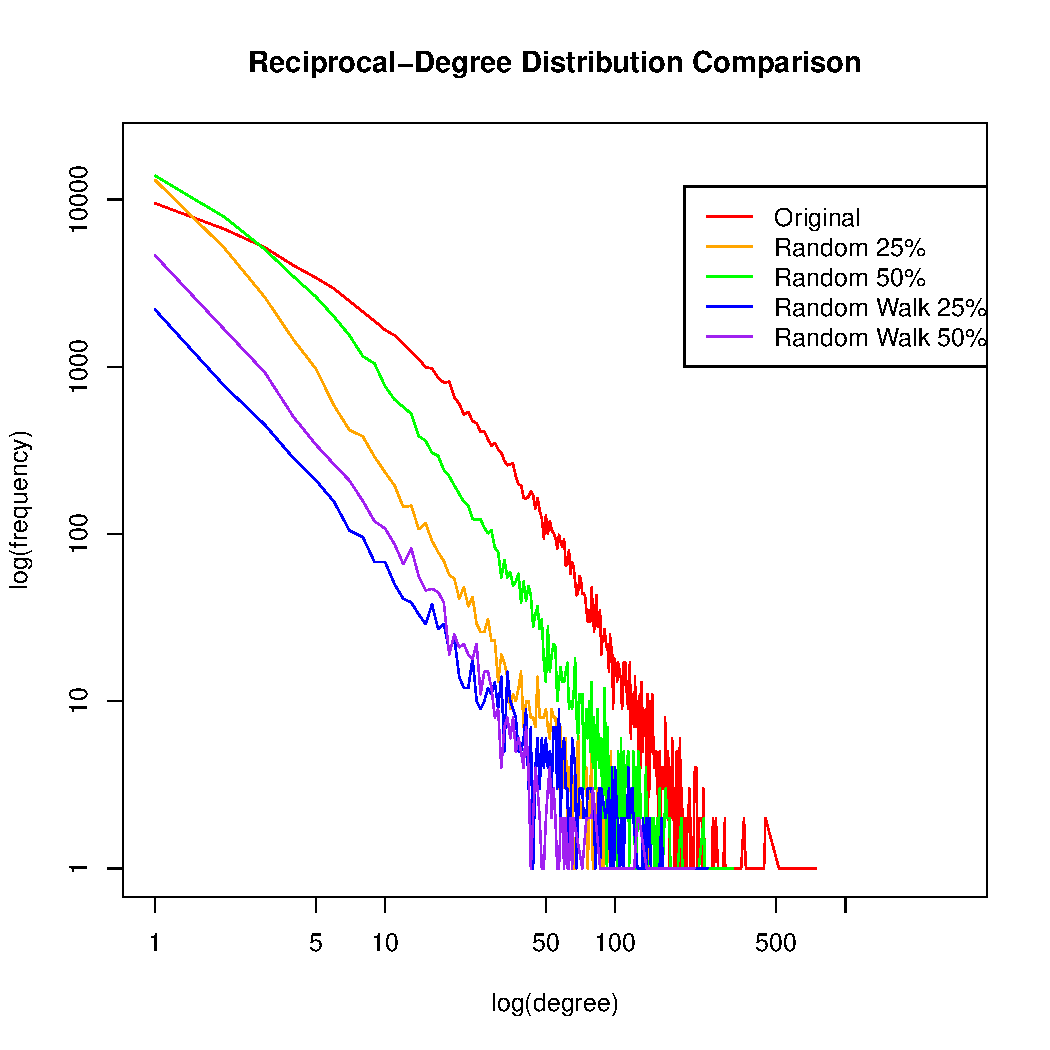
\includegraphics[width=\columnwidth]{subsampleComparison_recipDeg.pdf} 
\caption{Comparison of Reciprocal Degree Distributions for Sub-Samples \label{fig:ssRecipDeg}}
\end{figure}

\begin{figure}[h!]
\centering
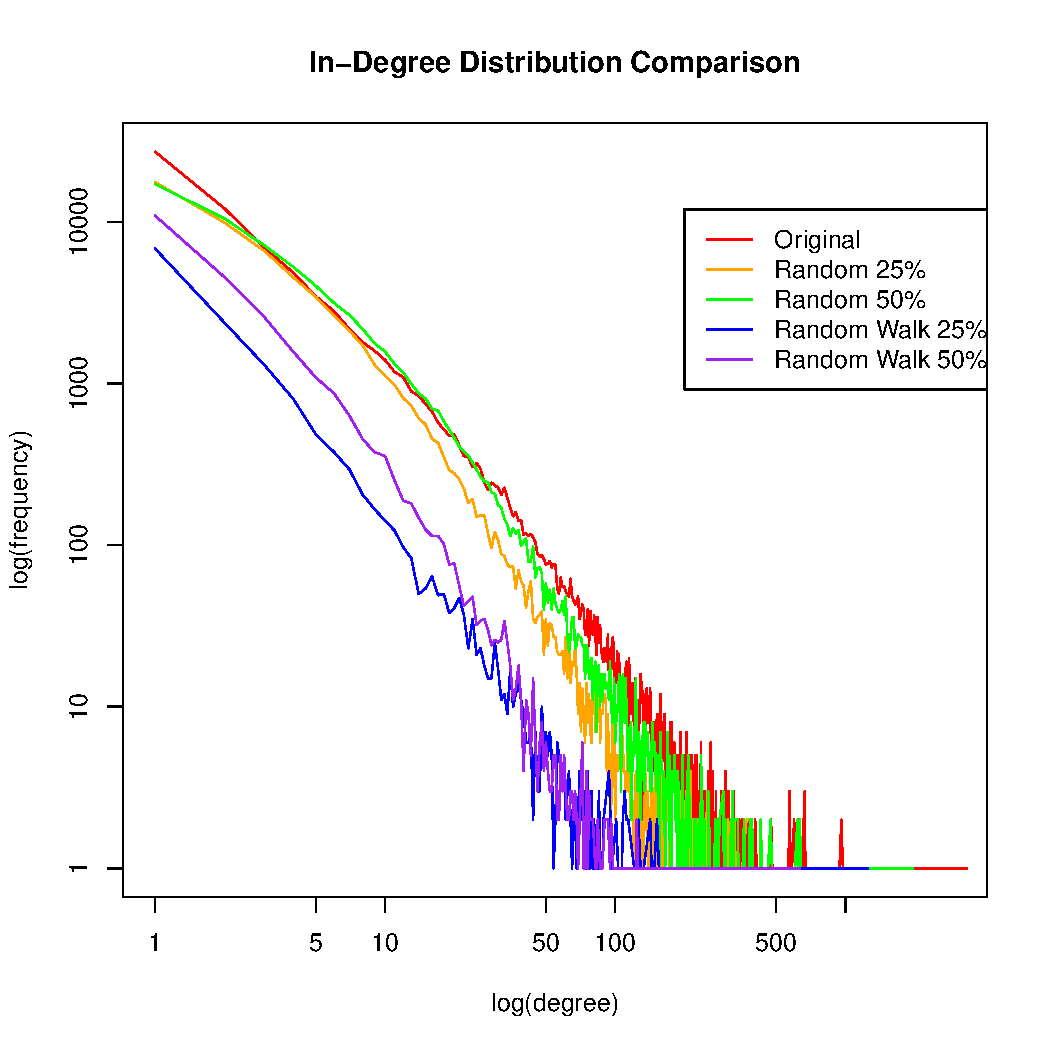
\includegraphics[width=\columnwidth]{subsampleComparison_inDeg.pdf} 
\caption{Comparison of In Degree Distributions for Sub-Samples \label{fig:ssInDeg}}
\end{figure}

\pagebreak

\begin{figure}[h!]
\centering
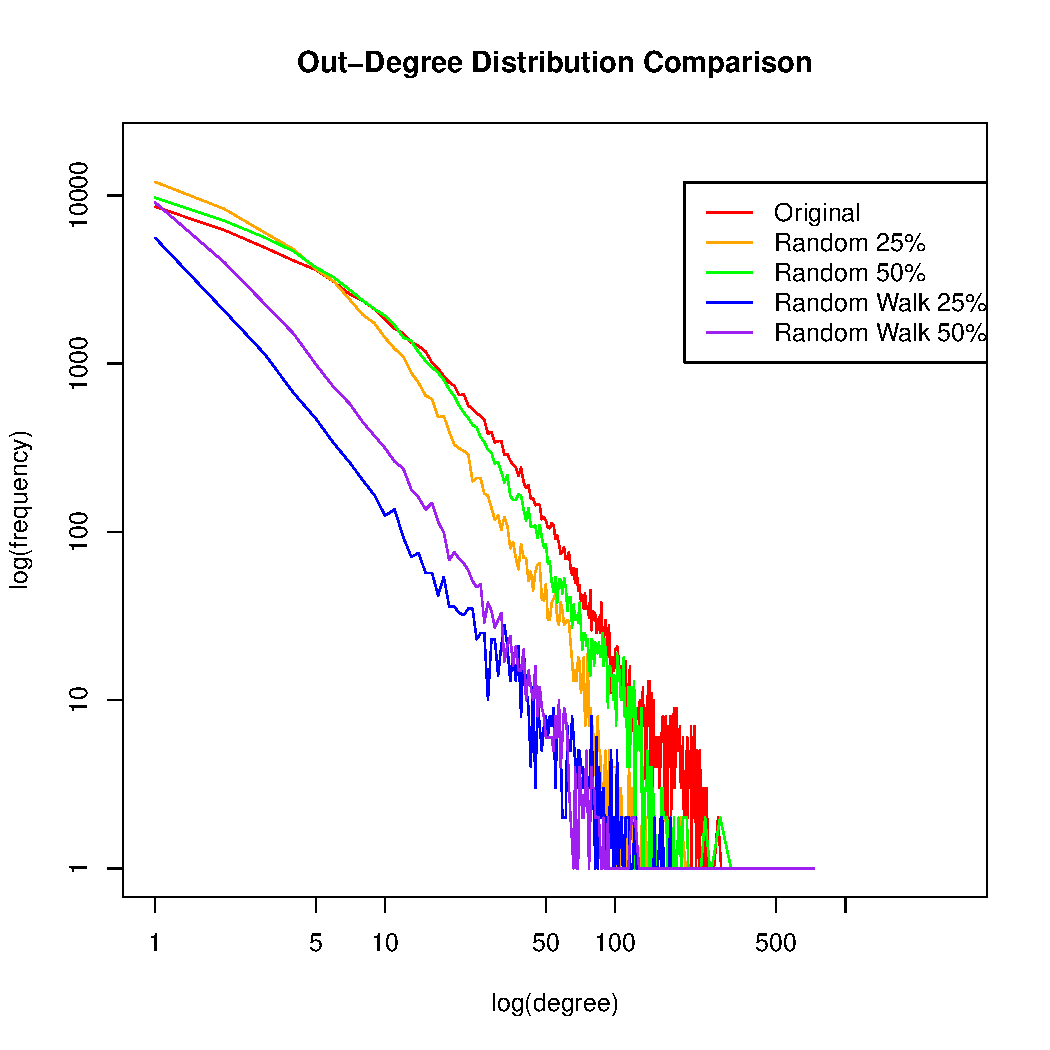
\includegraphics[width=\columnwidth]{subsampleComparison_outDeg.pdf} 
\caption{Comparison of Out Degree Distributions for Sub-Samples \label{fig:ssOutDeg}}
\end{figure}


% clustering 

\begin{figure}[h!]
\centering
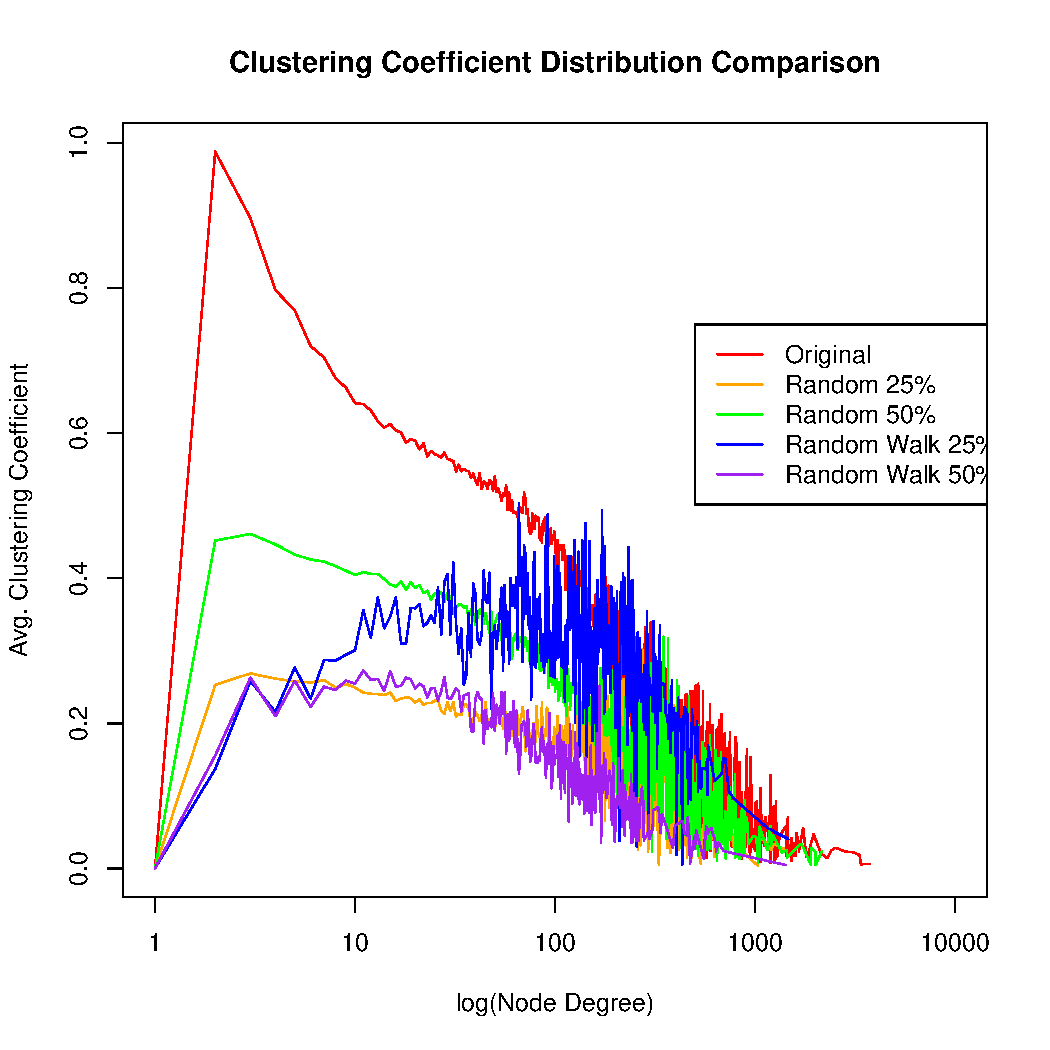
\includegraphics[width=\columnwidth]{subsampleComparison_clustering.pdf} 
\caption{Comparison of Clustering Distributions for Sub-Samples \label{fig:ssCluster}}
\end{figure}

% hop plots

\pagebreak

\begin{figure}[h!]
\centering
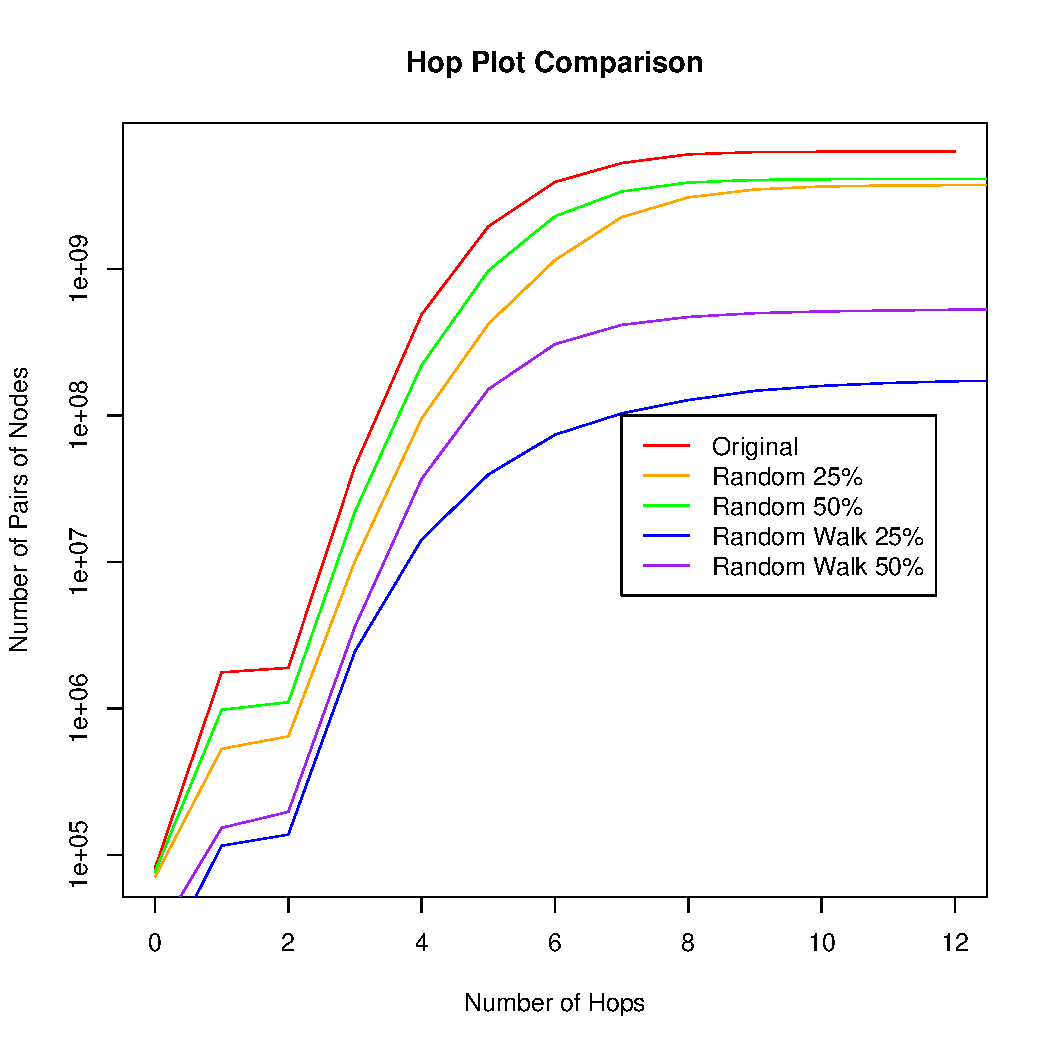
\includegraphics[width=\columnwidth]{subsampleComparison_hop.pdf} 
\caption{Comparison of Hop Plots for Sub-Samples \label{fig:ssHop}}
\end{figure}


\subsubsection{Generation Methods}
\label{sec:genFigures} 

\begin{figure}[h!]
\centering
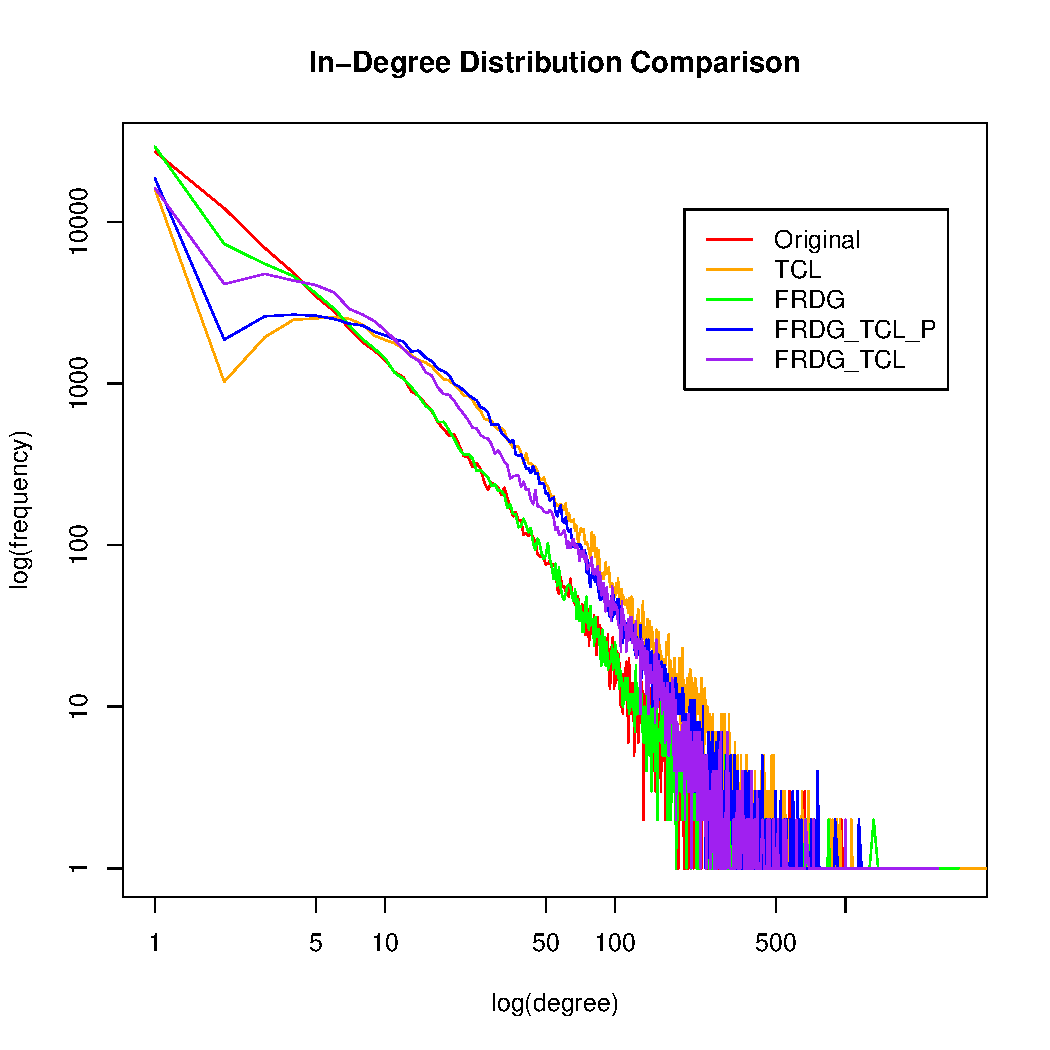
\includegraphics[width=\columnwidth]{generatedComparison_inDeg.pdf} 
\caption{Comparison of In Degree Distributions for Generated Graphs \label{fig:genInDeg}}
\end{figure}

\pagebreak

\begin{figure}[h!]
\centering
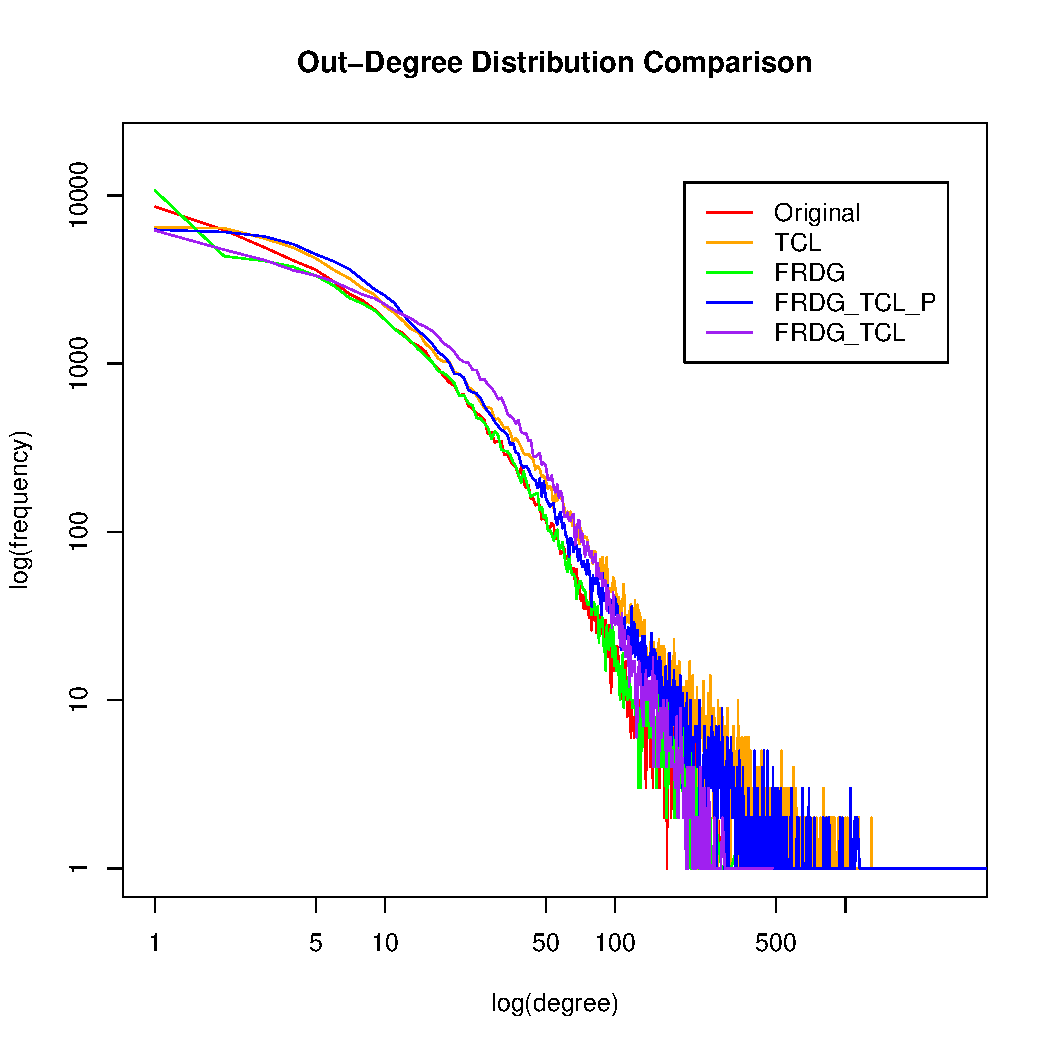
\includegraphics[width=\columnwidth]{generatedComparison_outDeg.pdf} 
\caption{Comparison of Out Degree Distributions for Generated Graphs \label{fig:genOutDeg}}
\end{figure}

\begin{figure}[h!]
\centering
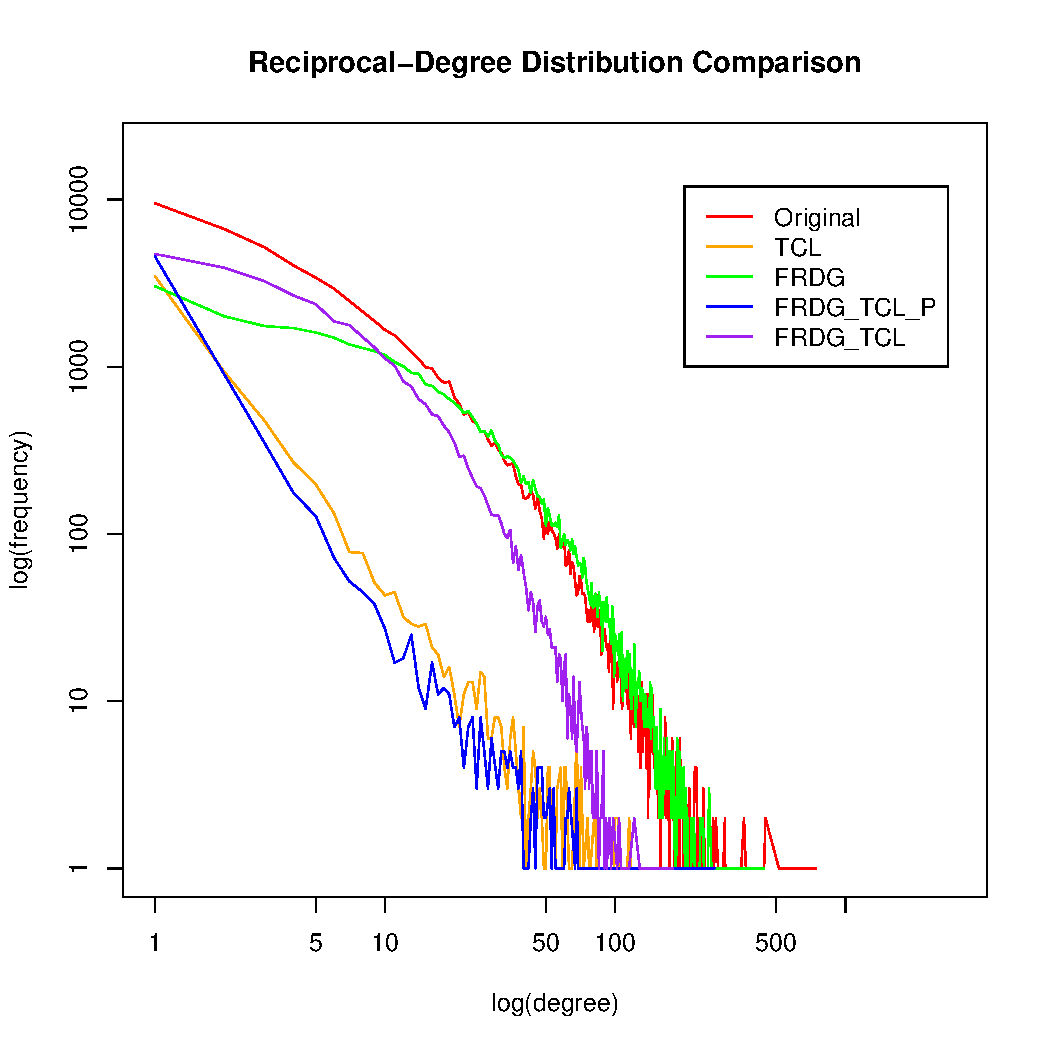
\includegraphics[width=\columnwidth]{generatedComparison_recipDeg.pdf} 
\caption{Comparison of Reciprocal Degree Distributions for Generated Graphs \label{fig:genRecipDeg}}
\end{figure}

\pagebreak

\begin{figure}[h!]
\centering
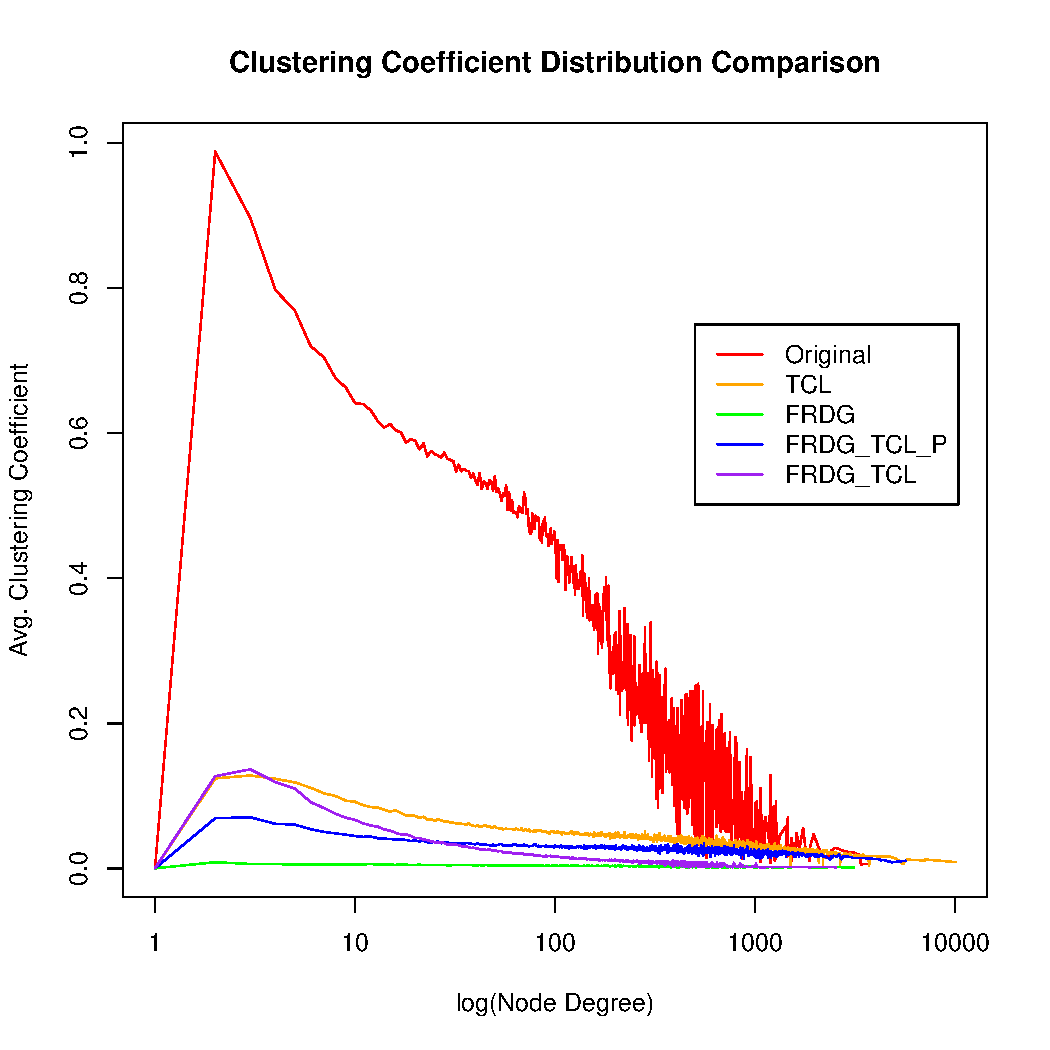
\includegraphics[width=\columnwidth]{generatedComparison_clustering.pdf} 
\caption{Comparison of Clustering Distributions for Generated Graphs \label{fig:genCluster}}
\end{figure}

\begin{figure}[h!]
\centering
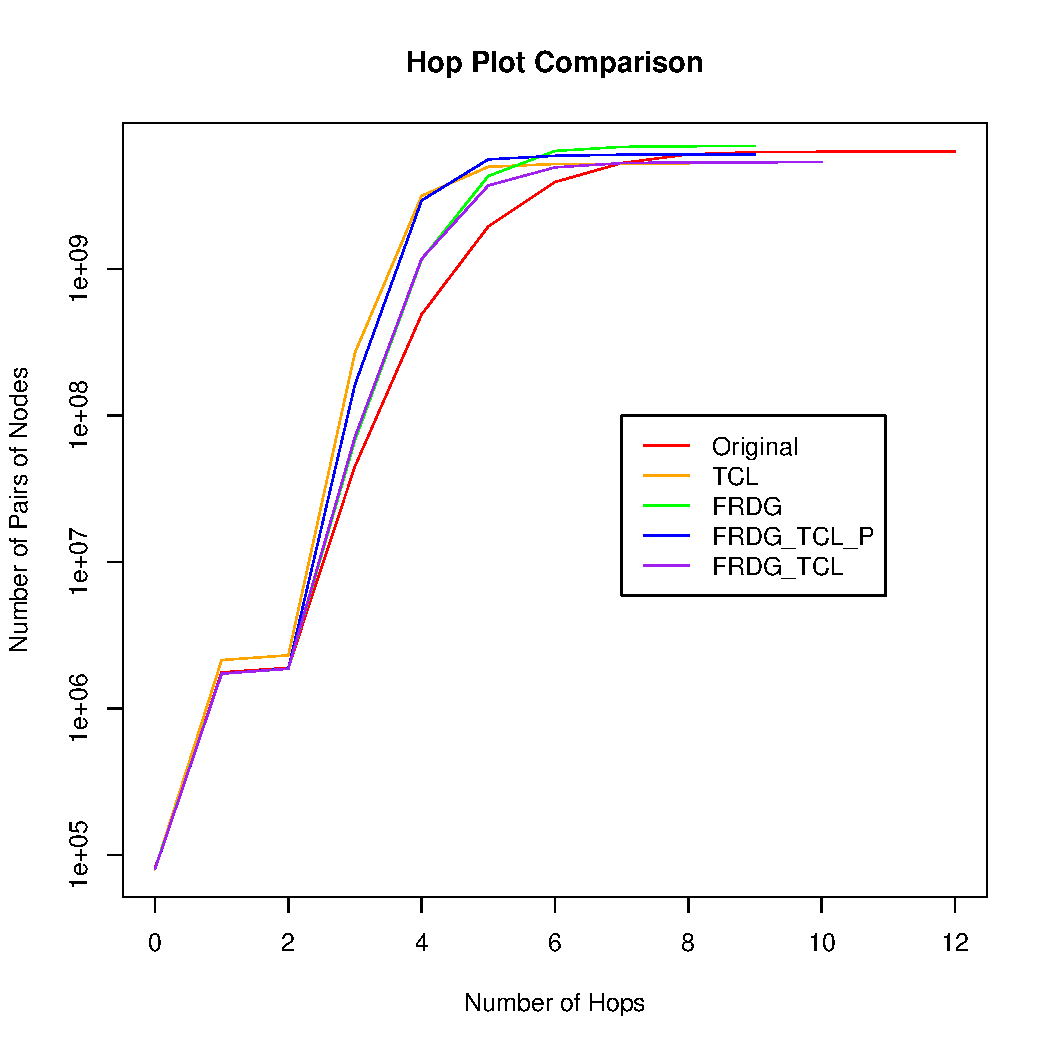
\includegraphics[width=\columnwidth]{generatedComparison_hop.pdf} 
\caption{Comparison of Hop Plots for Generated Graphs \label{fig:genHop}}
\end{figure}

\pagebreak

\subsubsection{Generated-from-Best-Sub-Sample Figures}
\label{sec:bestsFigures}

\begin{figure}[h!]
\centering
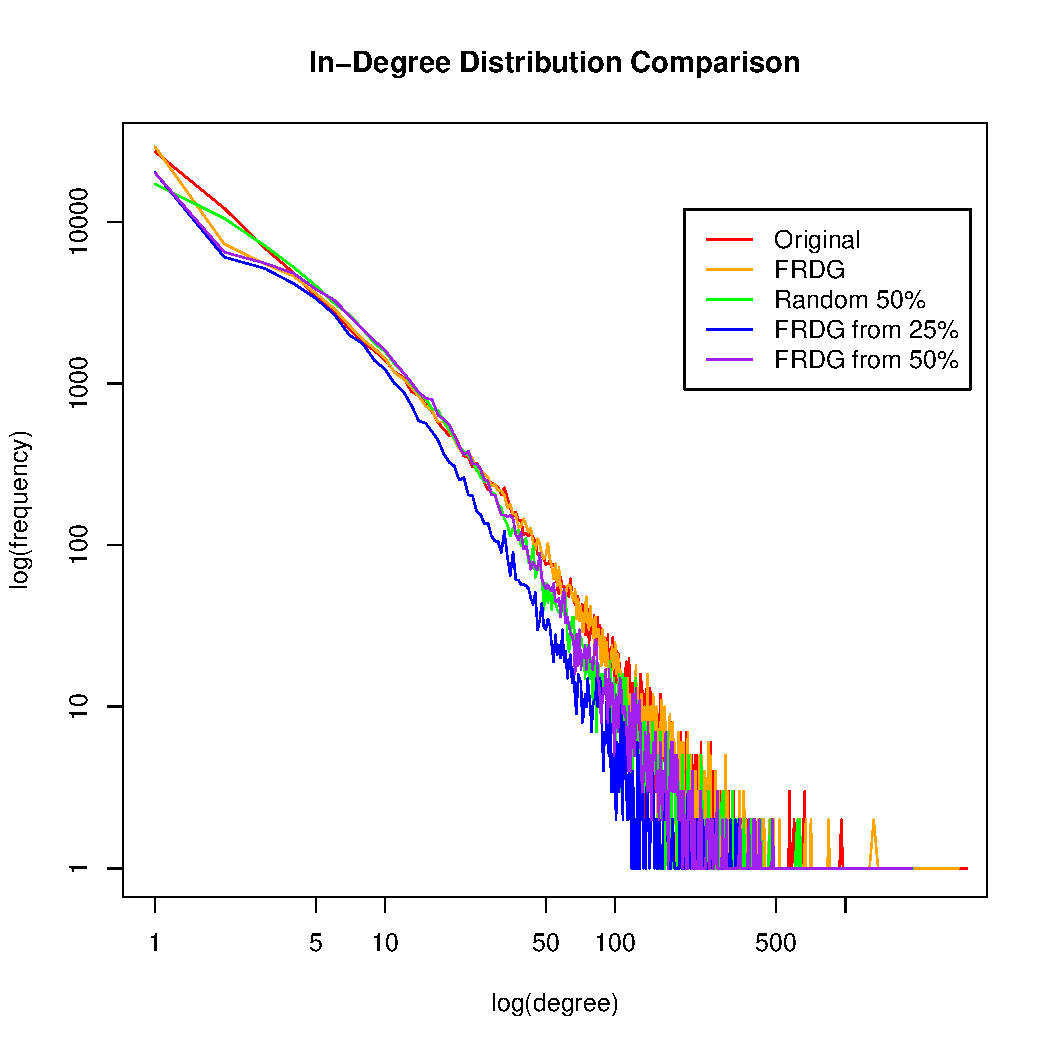
\includegraphics[width=\columnwidth]{bestsComparison_inDeg.pdf} 
\caption{Comparison of In Degree Distributions \label{fig:bestInDeg}}
\end{figure}

\begin{figure}[h!]
\centering
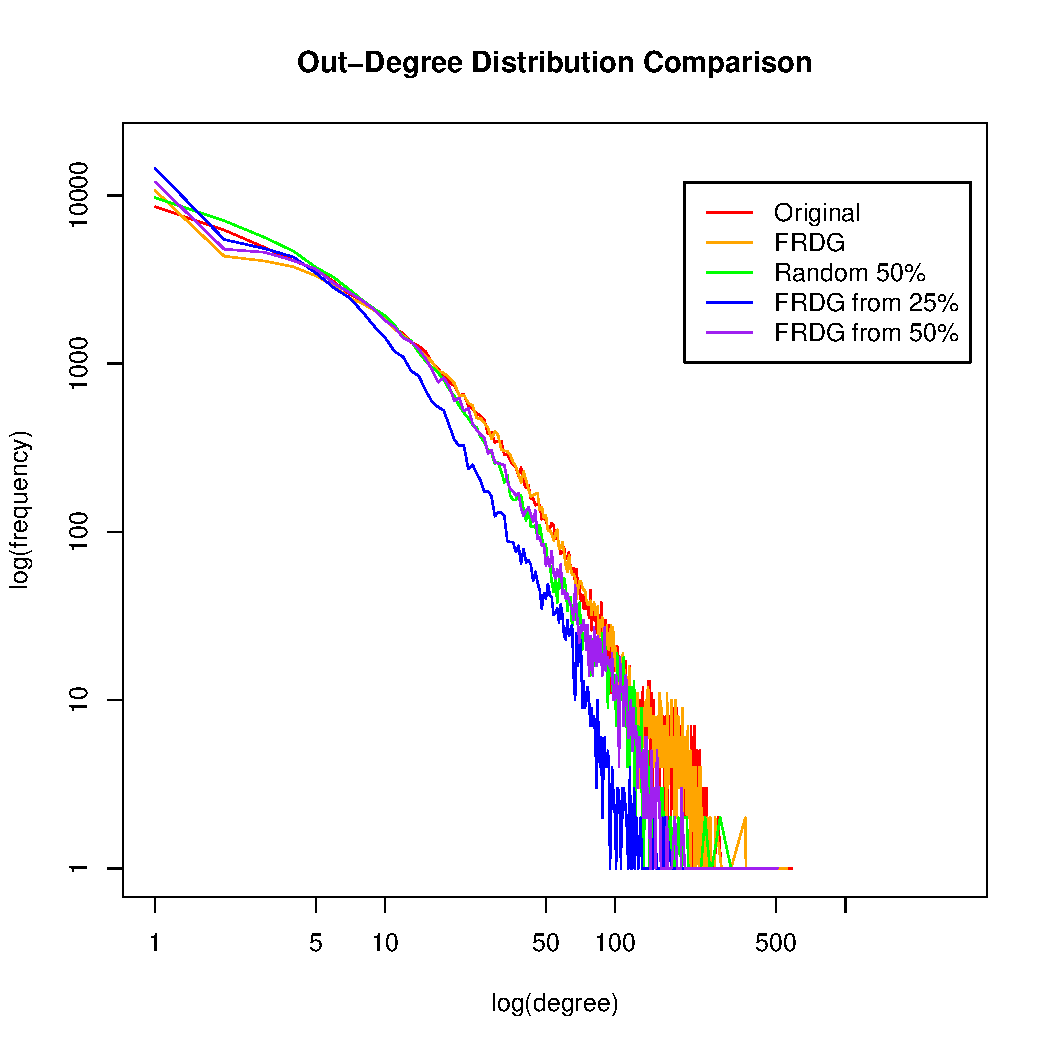
\includegraphics[width=\columnwidth]{bestsComparison_outDeg.pdf} 
\caption{Comparison of Out Degree Distributions \label{fig:bestOutDeg}}
\end{figure}

\pagebreak

\begin{figure}[h!]
\centering
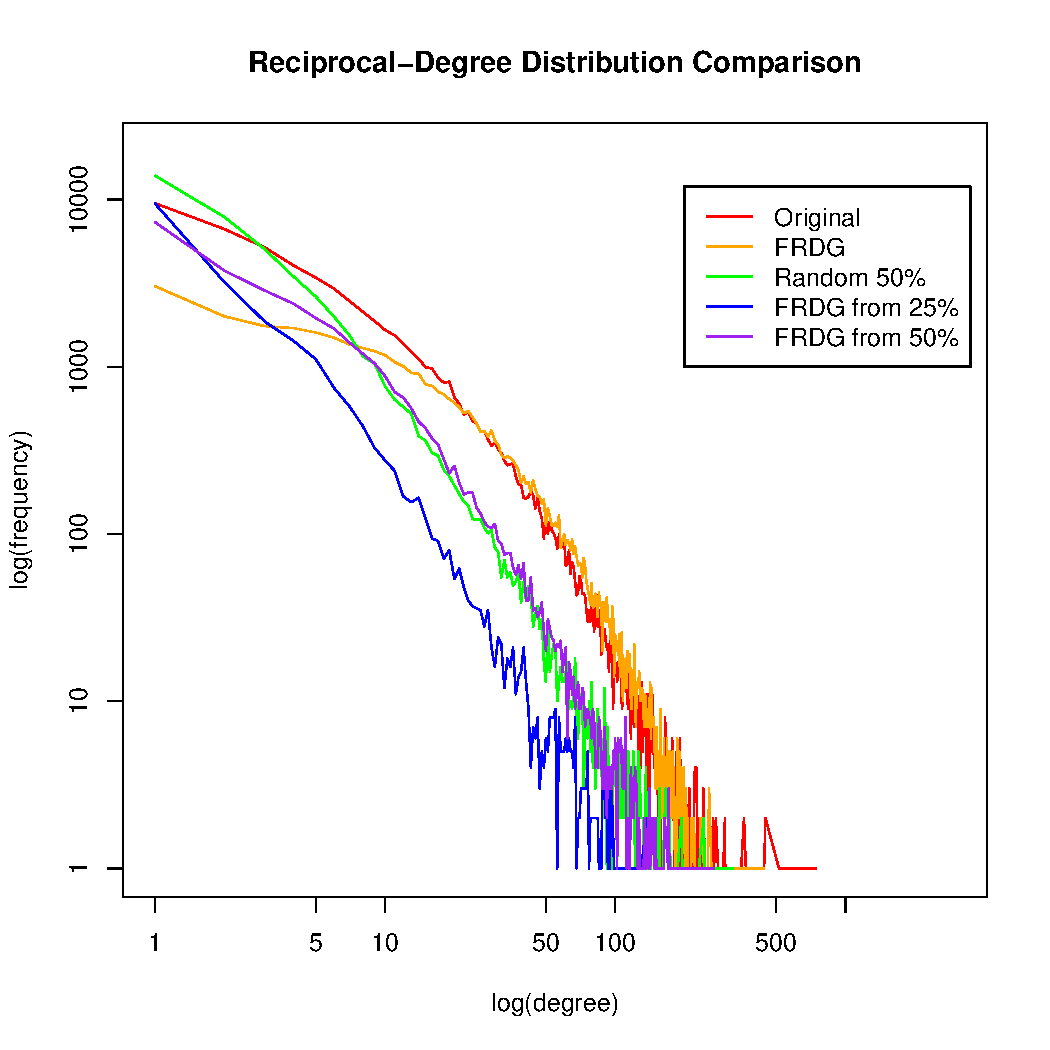
\includegraphics[width=\columnwidth]{bestsComparison_recipDeg.pdf} 
\caption{Comparison of Reciprocal Degree Distributions \label{fig:bestRecipDeg}}
\end{figure}

\begin{figure}[h!]
\centering
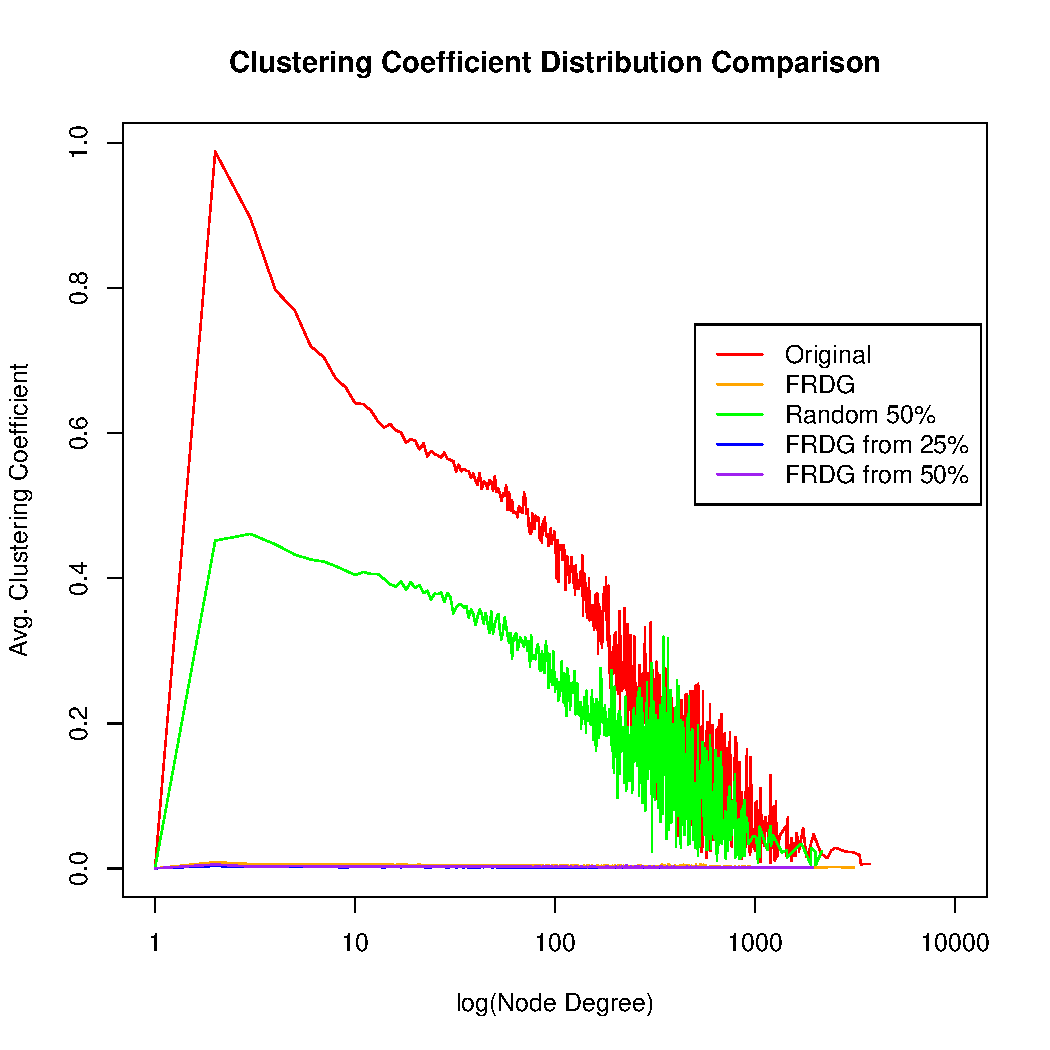
\includegraphics[width=\columnwidth]{bestsComparison_clustering.pdf} 
\caption{Comparison of Clustering Distributions \label{fig:bestCluster}}
\end{figure}

\pagebreak

\begin{figure}[h!]
\centering
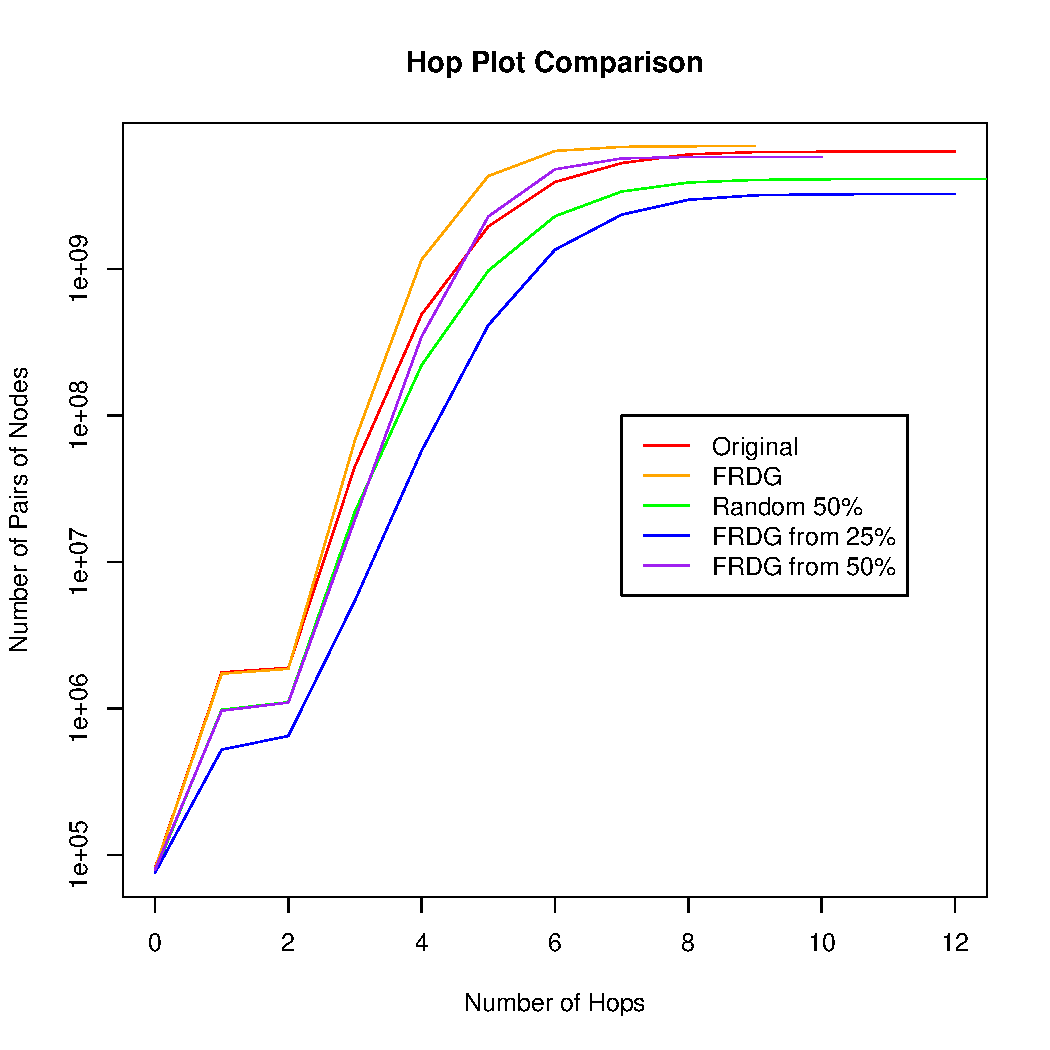
\includegraphics[width=\columnwidth]{bestsComparison_hop.pdf} 
\caption{Comparison of Hop Plots \label{fig:bestHop}}
\end{figure}

\pagebreak


\onecolumn
\subsection{Tables}
\label{sec:tables}

%\subsubsection{Full Sub-Sample Results}

\begin{table}[h]
\centering
\resizebox{.91\columnwidth}{!}{
\begin{tabular}{|l|l|cc|cc|cc|cc|}
\hline
Graph & Type & Nodes & Error & Edges & Error &	Average & Error & Average &	Error \\
&&&&&&Degree&&Clustering Coeff.&\\
\hline
Original & Original & 81306 & & 1768149 & & 43.5 & & 0.565 &	\\
\hline
RW-25 & Sub-Sample & 14845 & 0.817 & 115974 & 0.934 & 15.6 & 0.641 & 0.212 &	0.626\\
RW-50 & Sub-Sample &  26795 & 0.670 & 144092 & 0.919 & 11.5 & 0.736 & 0.195 & 0.655\\
Rand-25 & Sub-Sample &  70931 & 0.128 & 531032 & 0.700 & 15 & 0.655 & 0.208 & 0.632\\
Rand-50 & Sub-Sample & 77163 & 0.051 & 981492 & 0.445 & 25.4 & 0.416 & 0.354 & 0.374\\
\hline
TCL & Generated & 80155 & 0.014 & 2142624 & 1.175 & 53.5 & 0.187 & 0.075 & 0.867\\
FRDG & Generated & 80776 & 0.007 & 1730617 & 0.021 & 42.8 & 0.016 & 0.004 & 0.992\\
FRDG-Rand-25 & Generated & 75718 & 0.069 & 525348 & 0.703 & 13.9 & 0.680 & 0.002 & 0.997\\
FRDG-Rand-50 & Generated & 79227 & 0.026 & 967895 & 0.452 & 24.4 & 0.439 & 0.003 & 0.996\\
FRDG\_TCL\_FIXP & Generated & 80307 & 0.012 & 1730617 & 0.039 & 43.1 & 0.009 & 0.040 & 0.928\\
FRDG\_TCL & Generated & 80374 & 0.011 & 1730617 & 0.076 & 43.1 & 0.009 & 0.048 & 0.916\\
\hline
\end{tabular}
}
\caption{Characteristics of all Graphs by Type}
\label{table:NetChar}
\end{table}

% SCC = Strongly Connected Component
\begin{table}[h]
\centering
\resizebox{\columnwidth}{!}{
\begin{tabular}{|l|l|cc|cc|cc|cc|}
\hline
Graph & Type & Reciprocal & Error & Reciprocal & Error & Largest & Fraction & Largest & Fraction \\
 & & Edges & & Percentage & & SCC Nodes & of Nodes & SCC Edges & of Edges\\
\hline
Original & Original & 851692 & & 0.482 & & 68413 & 0.841 & 1685163 & 0.953 \\
\hline
RW-25 & Sub-Sample & 42046 & 0.951 & 0.363 & 0.247 & 11865 & 0.799 & 110599 & 0.953 \\
RW-50 & Sub-Sample & 40520 & 0.952 & 0.281 & 0.416 & 22230 & 0.830 & 144092 & 1.000 \\
Rand-25 & Sub-Sample & 102012 & 0.880 & 0.192 & 0.601 & 44837 & 0.632 & 458076 & 0.863 \\
Rand-50 & Sub-Sample & 292764 & 0.656 & 0.298 & 0.381 & 58279 & 0.755 & 905312 & 0.922 \\
\hline
TCL & Generated & 29861 & 0.965 & 0.014 & 0.971 & 68299 & 0.852 & 2052125 & 0.958 \\
FRDG & Generated & 819694 & 0.017 & 0.474 & 0.017 & 67803 & 0.839 & 1577568 & 0.912 \\
FRDG-Rand-25 & Generated & 97138 & 0.886 & 0.185 & 0.616 & 44302 & 0.585 & 316693 & 0.603 \\
FRDG-Rand-50 & Generated & 281050 & 0.670 & 0.290 & 0.397 & 60324 & 0.761 & 778330 & 0.804 \\
FRDG\_TCL\_FIXP & Generated & 19795 & 0.976 & 0.011 & 0.976 & 71172 & 0.886 & 1667138 & 0.963 \\
FRDG\_TCL & Generated & 314632 & 0.631 & 0.182 & 0.622 & 68734 & 0.855 & 1596243 & 0.922 \\
\hline
\end{tabular}
}
\caption{Connection results of all Graphs by Type}
\label{table:NetResults}
\end{table}

\begin{table}[h]
\centering
\resizebox{.7\columnwidth}{!}{
\begin{tabular}{|l|l|ccc|}
\hline
Graph & Type & Diameter & $90\%$ Effective Diameter & SCC Diameter \\
\hline
Original & Original & 14 & 15 & 14 \\
\hline
RW-25 & Sub-Sample & 31 & 31 & 29 \\
RW-50 & Sub-Sample & 27 & 28 & 26  \\
Rand-25 & Sub-Sample & 26 & 24 & 23 \\
Rand-50 & Sub-Sample & 22 & 22 & 22 \\
\hline
TCL & Generated & 10 & 10 & 10 \\
FRDG & Generated & 14 & 15 & 14  \\
FRDG-Rand-25 & Generated & 20 & 20 & 19 \\
FRDG-Rand-50 & Generated & 15 & 15 & 14 \\
FRDG\_TCL\_FIXP & Generated & 12 & 12 & 12 \\
FRDG\_TCL & Generated & 15 & 15 & 15  \\
\hline
\end{tabular}
}
\caption{Diameters of all Graphs by Type}
\label{table:NetDiameter}
\end{table}


\pagebreak

\subsection{Code}
All code and project content can be viewed and modified at \url{https://github.com/pdsteele/socialNetworksProject/}

%\addcontentsline{toc}{subsubsection}{Code}
\subsubsection{Transitive Chung-Lu Code}
\label{sec:TCL}
\lstinputlisting[language=Python]{proj-TransChungLu.py}

\pagebreak

\subsubsection{Fast Reciprocal Directed Graph}
\label{sec:FRDG}
\lstinputlisting[language=Python]{proj-fastRecipDirGraph.py}

\pagebreak

\subsubsection{Twitter Sub-Sampling and Data Reformatting}
\label{sec:subsampleCode}
\lstinputlisting[language=Python]{proj-convert_Twitter.py}

\pagebreak

\subsubsection{SNAP Graph Conversion Code}
\label{sec:readData}
\lstinputlisting[language=C]{proj-readInData.cpp}

\pagebreak

\subsubsection{SNAP Stat Calculation Code}
\label{sec:calcStats}
\lstinputlisting[language=C]{proj-calcStats.cpp}

\pagebreak

\subsubsection{Degree Distribution Calculation Code}
\label{sec:degreeDistros}
\lstinputlisting[language=Python]{proj-degreeDistros.py}

\pagebreak




\end{document}